% ----------------------------------------------
% IT2901 - Informatikk Prosjektarbeid II
% Norwegian University of Science and Technology
% ----------------------------------------------

\documentclass[11pt,a4paper,twoside]{report}
%\setlength{\oddsidemargin}{5mm}
%\setlength{\evensidemargin}{25mm}
\usepackage{geometry}
%[top=4.cm, bottom=4.5cm, left=3.cm, right=3.cm]
\usepackage{lumalayout}       % Custom fancy layout fra hælvette
\usepackage[utf8]{inputenc}	  % Unicode for norske tegn
\usepackage[pdftex]{graphicx} % Støtte for bilder inkl. pdf
\usepackage{nameref}          % Støtte for labels på kapittel og seksjoner
\usepackage{wrapfig}	%wrapfigure
\usepackage[table]{xcolor}
\usepackage{colortbl}         % Kolonne farge i tabeller
\usepackage{multirow}
\usepackage{parskip}
\usepackage{tabularx}
\usepackage{umoline}
\usepackage{pifont}
\usepackage{listings}
\usepackage{float}
\usepackage{caption}
\usepackage{appendix}
\usepackage{fixltx2e}
\usepackage{color}
\usepackage{xcolor}
\usepackage[none]{hyphenat}
\usepackage{hyperref}         % Lenker !! Må være til slutt !!
\usepackage[xindy]{glossaries}

% Custom commands ------------------------------------------------------------ %
% Her kan vi legge inn kommandoer for ord og uttrykk, som forekommer ofte i
% rapporten. På den måten får vi uttrykt oss mer konsistent gjennom rapporten, 
% pluss at det blir enklere for oss å forandre på formatteringen av viktige ord
% underveis (f.eks at vi plutselig bestemmer oss for at ntnu skal skrives i
% kursiv eller med fet skrift).
%
% Vi kan prøve å følge en konvensjon her også. Et forslag:
%
%     Kommandoer med små bokstaver -> Full beskrivelse av ordet/uttrykket
%     Kommandoer med store bokstaver -> Forkortelser
%
% Eksempel: 
%
%    \ntnu -> Norwegian University of Science and Technology
%    \NTNU -> NTNU

\newcommand{\project}{oSNAP}

\newcommand{\HRule}{\rule{\linewidth}{0.5mm}}

\newcommand{\todo}[1]{\textbf{[TODO: {\color{red}#1}]}}

% Names
\newcommand{\anders}{\mbox{Anders \textsc{B. Eie}}}
\newcommand{\asbjorn}{\mbox{Asbjørn \textsc{Lucassen}}}
\newcommand{\bjornar}{\mbox{Bjørnar \textsc{Håkenstad Wold}}}
\newcommand{\emanuele}{\mbox{Emanuele \textsc{Di Santo}}}
\newcommand{\henrik}{\mbox{Henrik \textsc{Goldsack}}}
\newcommand{\johan}{\mbox{Johan \textsc{Jansen}}}
\newcommand{\jonas}{\mbox{Jonas \textsc{Svarvaa}}}

%\newcommand{\redcell}[1]{\cellcolor{red!80!yellow}#1}
%\newcommand{\grncell}[1]{\cellcolor{green!40!yellow}#1}
%\newcommand{\ylwcell}[1]{\cellcolor{yellow}#1}

% Custom settings ------------------------------------------------------------ %
% listings defitions
\definecolor{javared}{rgb}{0.6,0,0} % for strings
\definecolor{javagreen}{rgb}{0.25,0.5,0.35} % comments
\definecolor{javapurple}{rgb}{0.5,0,0.35} % keywords
\definecolor{javadocblue}{rgb}{0.25,0.35,0.75} % javadoc

\newcommand{\javacode}{\lstset{language=Java,
basicstyle=\scriptsize\ttfamily,
keywordstyle=\color{javapurple}\bfseries,
stringstyle=\color{javared},
commentstyle=\color{javagreen},
morecomment=[s][\color{javadocblue}]{/**}{*/},
numbers=left,
numberstyle=\tiny\color{black},
stepnumber=1,
numbersep=4pt,
tabsize=4,
showspaces=false,
showstringspaces=false,
breaklines=true}}

\newcommand{\ccode}{\lstset{language=C++,
basicstyle=\scriptsize\ttfamily,
keywordstyle=\color{Blue},
stringstyle=\color{BurntOrange},
commentstyle=\color{Gray},
numbers=left,
numberstyle=\tiny\color{black},
stepnumber=1,
numbersep=10pt,
tabsize=4,
showspaces=false,
showstringspaces=false,
breaklines=true}}


\DeclareGraphicsExtensions{.pdf, .png, .jpg, .gif}
\graphicspath{{./img/}}

\setlength{\headheight}{15pt}
\setcounter{tocdepth}{3}
\hypersetup{colorlinks=true, 
			linkcolor=black, 
			filecolor=black,
			citecolor=black,
			urlcolor=black}

\input{./files/glossary}
\makeglossaries

\geometry{bindingoffset=2cm}
\begin{document}

% ---------------------------------------------------------------------------- %
% Title page, table of contents, list of tables and figures goes here

\begin{titlepage}
	\begin{center}
		
\includegraphics[width=0.75\textwidth]{img/NTNU-logo.png}\\[1cm]    
		\textsc{\Large IT2901 - Informatics Project II}\\[0.5cm]
		\HRule \\[0.6cm]
		{ \huge \bfseries \project}\\[0.4cm]
		open Social Network Arduino Platform
		\HRule \\[1.5cm]
		\begin{center} \large
			\anders \\
			\henrik \\
			\johan \\
			\asbjorn \\
			\emanuele \\
			\jonas \\
			\bjornar
		\end{center}
		\vfill
		{\large \today}
	\end{center}
\end{titlepage}


%Abstract
%An experienced reader should be able to understand 
%exactly what you have done from only reading the 
%abstract:
% - This is different from a summary.  
% - Should be short, varies from 150 to 200 word maximum 
% - Should include a description of the problem, the solution and the main results. 
% - Typically the last thing you write
\begin{abstract}
This is our abstract. Last thing we will write.
\end{abstract}

\cleardoublepage
\tableofcontents
\cleardoublepage

\listoffigures
\cleardoublepage

\listoftables


%\printglossaries
%\newpage

% ---------------------------------------------------------------------------- %
% Main report body goes here
\cleardoublepage
\chapter{Introduction}\label{ch:introduction}
\section{Problem description}

\emph{This is the problem description, as per the customer's request.}

Social networking sites such as Facebook and Twitter have normally been accessed  via a web browser.
Lately mobile versions have become popular, and allow access to context data such as location of
users. We foresee a much greater popularity of mobile and pervasive interfaces to social media in
the coming years.

Arduino\cite{link:arduino} is a platform that allows software to be written in order to construct
hardware prototypes. In this task the students will develop an Arduino-based interface to Facebook.
The information from Facebook will be made available on Arduino displays and the user can interact
with Facebook through Arduino sensors and actuators.

In case Facebook data access shows to be difficult, the students will use Shindig\cite{link:shinding} which 
is an open source implementation of OpenSocial APIs. The service specification is developed in the European project 
SOCIETIES in collaboration with European partners. The students are however expected to innovate and come up 
with new concepts, user interfaces, and service organization.

\section{The context}
In the past few years, social networks have become more and more popular, continuously increasing their userbase.
The project task was to design and develop an open source Android\cite{link:android} framework for allowing quick
and flexible development of wireless Tangible User Interfaces (T.U.I.) for social networks using Arduino.
The product has served both as a proof-of-concept and as a starting point for future software projects.

\section{The customer}
Our customer was SINTEF, represented by Mr. Babak A. Farshchian.

SINTEF is the largest independent research organisation in Scandinavia \cite{link:sintef}.
It is an independent, non-commercial organisation with their head office in Trondheim. They have approximately 2100 employees, mainly in Trondheim and Oslo.

\section{The team}
The team consisted of seven students from NTNU. About half of the members have worked
together on previous projects and thus shared some teamwork skills and experiences.
Having a properly functioning team where all the skills of each team member are properly
utilized is vital for the success of any project. None of the team members had 
worked for a customer before.

\subsection{Team members}

\begin{itemize}
\item{\anders}\newline
Third year Informatics student at NTNU. Experience with the programming languages Java,
C and C++. Also experience with Arduinos, AVRs and some basic electronics knowledge.

\item{\henrik}\newline
Third year student at NTNU. Main language Java, basic knowledge in 3D and electronic circuits.

\item{\johan}\newline
Third year student at NTNU. Experience with the programming languages Java, C, C++  and
Basic. Worked with AVR microcontrollers in other projects and courses.

\item{\asbjorn}\newline
Second year student on bachelor in computer science at NTNU. Has previously had one year of
introductory psychology which is to be included in the bachelor in computer science.
Experience with Java.

\item{\emanuele}\newline
Third year Computer Science exchange student from Tor Vergata University, Rome.
Experience with Java, C and C++ programming.

\item{\jonas}\newline
Third year student at NTNU. Experience with Java, Python, Lua, PHP, and web standards such as HTML,
CSS and Javascript. Previously worked with media and sound engineering.

\item{\bjornar}\newline
Third year Informatics student at NTNU. Experience with programming in Java, C and C++.
Previously worked with electronics and have basic knowledge about AVR microcontrollers through
own projects.
\end{itemize}

\section{Definitions}

Here we introduce a list of the terms used in this document with a short explanation of their meaning.

\begin{description}
\item[Facebook] Facebook is the biggest social network. It is also the network our libraries primarily focus on.
\item[OpenSocial] OpenSocial\cite{link:opensocial} is an open source standard by Google for a set of API. It's aim is to
provide a common runtime environment for web applications within different social networks. It is supported by networks
such as Orkut, MySpace, LinkedIn and many more. Facebook and Twitter do not support OpenSocial and they both have their
own custom propietary APIs.
\item[Apache] A software foundation focused on open source and community driven software.
\item[Shindig] Shindig is Apache's implementation of the OpenSocial standard.
\item[Android] A operating system based on Linux primarily for mobile devices made by Google.
\item[Arduino] Arduino is a tool for making computers that can sense and control more of the physical world than your
desktop computer. It's an open-source physical computing platform based on a simple microcontroller board, and a development
environment for writing software for the board. \cite{link:arduino}
\item[Product] This project's deliverables: a set of prototypes and Android applications and libraries.
\item[Prototype] An Arduino board, running a custom firmware. It works in conjunction with an Android application
that controls its behaviour and another Android application that fetches the required data from a social network.
\item[Social service] With this term we refer to Android services used to fetch data from a social network.
\item[Android-Arduino applications] With this term we refer to Android applications used to control the behaviour of prorotypes.
\end{description}


\cleardoublepage
\chapter{Process Management}\label{ch:management}
\section{The Team}
The team consists of seven students from NTNU. About half of the members have worked
together on previous projects and therefore have experience functioning together as a
team. Having a properly functioning team where all the skills of each team member is properly
utilized is vital for the success of any project. None of the team members have any experience 
working for a customer so we have to prepare for any challenges this might cause.


%Roles of each member? Scrum Master, Team Leader, Customer Relations, etc.
\subsection{Project Roles}
Scrum Master: Henrik Goldsack\newline
Customer Relations: Henrik Goldsack\newline
Quality Assurance: ???\newline
Hardware Managment: Johan Jansen and Asbjørn Lucassen\newline

\todo 
{
describe each of the role... who is the Customer? mention the Student Assistant
}

\subsection{Emanuel Di-Santo}
???

\subsection{Anders Behne Eie}
Third year Informatics student at NTNU. Experience with the programming languages Java, C and C++. Also experience with Arduinos, AVRs and some basic electronics knowledge.

\subsection{Henrik Nicolai Goldsack}
???

\subsection{Johan Jansen} 
Third year student at NTNU. Experience with the programming languages Java, C, C++  and 
Basic. Worked with AVR microcontrollers in other projects and courses.

\subsection{Asbjørn Lucassen}
Second year student on bachelor in computer science at NTNU. Has previously had one year of introductory psychology which is to be included in the bachelor in computer science.
Experience with Java.

\subsection{Jonas Svarvaa}
Third year student at NTNU. Experience with Java, Python, Lua, PHP, and web standards such as HTML, CSS and Javascript. Previously worked with media and sound engineering.

\subsection{Bjørnar Håkenstad Wold}
Third year Informatics student at NTNU. Experince with programming in Java, C and C++. Previously worked with electronics and have basic knowledge about AVR microcontrollers through own projects.


\newpage
\section{Selecting Development Process}
Choosing a development process is crucial for every project as many varying factors such as
project size, members and time affect which process is suitable. The following section describes
which development processes we have considered using. The choice of the development method
will affect how the group communicates, collaborates and write the code.

\subsection{Waterfall}
The Waterfall model is a strict top-down design process. \cite{bib:waterfall}It features detailed planning, design and
documentation before design. The strict model is useful where going back and changing requirements is 
costly or impossible. This does however require that all needed features and requirements are known
early on. The model was originally used for hardware design and when the first software projects 
appeared it was simply adapted. Many argue that the Waterfall model is bad for software design, seeing
as the developers cannot predict all problems or additional requirements before reviewing a working
prototype of the final product. Customers also often have changing requirements under development.
The Waterfall model works best for expensive projects where problem prediction and initial correct design
is vital before implementation is started.
\begin{figure}[h!]
\centering 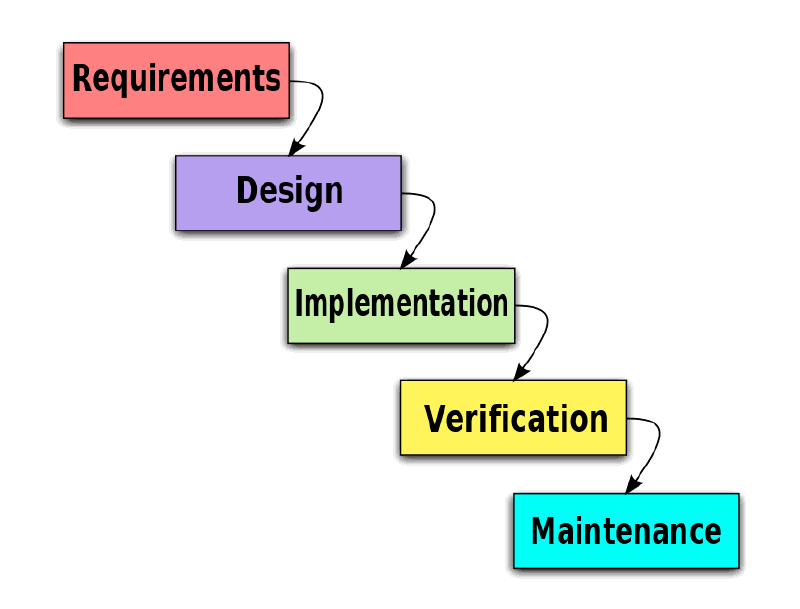
\includegraphics[scale=0.30]{img/designmodel-waterwall} \caption{The Waterfall model}
\label{fig:desigmodel-waterfall}
\end{figure}

\subsection{Scrum}
Scrum is a for of agile project managment. The scrum approach uses  repetitive iterations (called 
a Sprint in the Scrum etymology) to design, implement and refine a product. Each iteration improves,
fixes and adds new features to the previous iteration. A key feature of Scrum is that the customer
can change their mind on what they want or need. Scrum focuses on frequent group meetings and
splitting big tasks into lesser, managble tasks for smaller groups of programmers. Because of the
frequent meetings it promotes verbal communication in the group.
\begin{figure}[h!]
\centering 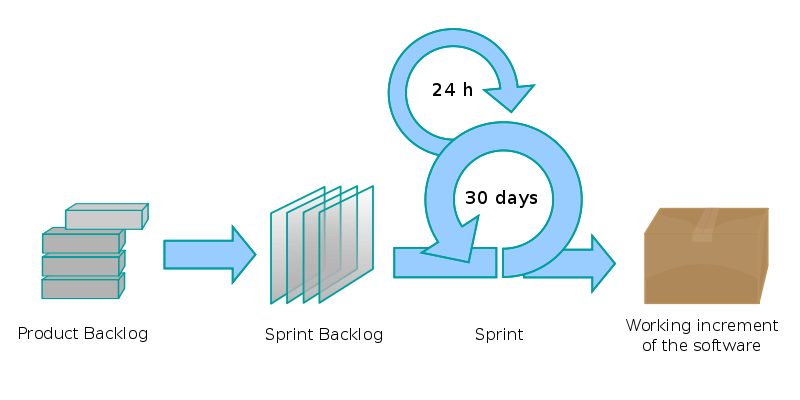
\includegraphics[scale=0.4]{img/designmodel-scrum} \caption{The Scrum process}
\label{fig:desigmodel-scrum}
\end{figure}

\subsection{Extreme Programming (XP)}
Extreme Programming is a development methodology that is designed for best software quality and
quick responsivness to changing customer requirements. It is also an Agile Development method like
Scrum and therefore shares certain similarities to that development method. It promotes rapid
development and allows the customer to change his/her mind or request new features throughout
the development of the software. Typical elements for XP are pair programming, unit testing,
lazy programming, simplicity and expecting changes in customer requirements as time passes
and the problem is better understood. Several pitfalls include buggy and unstable code or lack of
overall design specification. Extreme programming is best suited for small projects for prototyping
where the customer is not entierly sure what he or she wants.
\begin{figure}[h!]
\centering 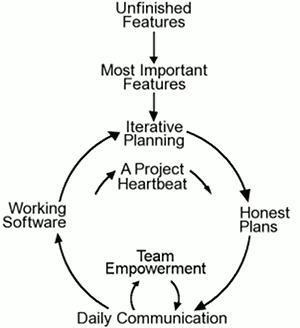
\includegraphics[scale=0.75]{img/designmodel-xp} \caption{Extreme Programming}
\label{fig:desigmodel-xp}
\end{figure}

\subsection{Agile Unified Process}
The AUP (short for Agile Unified Process) offers a simple and easy to understand approach for software
development. It is a simplified version of the Rational Unified Process. Key features are simplicity, 
customization and focus on the task on hand instead of everything that may or will happen. It features 
several internal development iterations before producing a customer release. AUP focuses on quality
insurance and works best for projects that is going to be used by a large public and a working, bugfree
product is important.
\begin{figure}[h!]
\centering 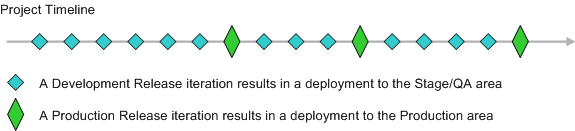
\includegraphics[scale=0.65]{img/designmodel-aup} \caption{AUP development iterations}
\label{fig:desigmodel-aupl}
\end{figure}

\subsection{Spiral Model}
The Spiral development methodology combines the advantages of both the top-down approach from 
Waterfall and the bottom-up concept of prototyping. It does this by using iterative development and
controlling it through the systematic Waterfall model. A strong advantage of the Spiral lifecycle is that it
allows new features and requests to be integrated as soon as they come avalible or known. Other key 
features of the model is risk analysis, strict sysem design specifications and prototyping. The Spiral model
 is best suited for large, expensive and complicated projects.
\begin{figure}[h!]
\centering 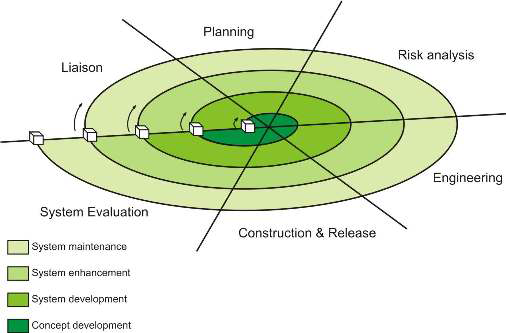
\includegraphics[scale=0.85]{img/designmodel-spiral} \caption{The Spiral model}
\label{fig:desigmodel-spiral}
\end{figure}

\subsection{Conclusion}
We initially selected Scrum as our development process. The arguments  for using Scrum were that we would
have a work schedule that fit into a iterative process in addition to weekly meetings with a customer that
wanted a new version of the prototype each sprint. Moreover everyone in the team had existing experience 
with Scrum from previous projects. After a few weeks of development however, we observed that the Scrum
model did not fit our project. Unspecific and unclear requirements from the customer lead along with
the customer wanting a working prototype from week 1 meant we had to change our entire development
process. This cost us a lot of work since we had already setup and planned the project using Scrum 
development methodology, but after each meeting of the customer the entire project goal changed. This
lead us into researching using either Extreme Programming or the Spiral model. But after the third week we
settled back into Scrum development.

\section{Project management tools}

To accompany us in the Scrum process we have chosen an online tool
called ScrumDo (www.scrumdo.com). This tool has features for most
if not all parts of the Scrum process. Using this tool consistently
will be our main method of maintaining and separating packages from
the WBS (Work Breakdown Structure). In the context of ScrumDo and
Scrum these low level work packages are called stories and are moved
accordingly from \char`\"{}ToDo\char`\"{} over to \char`\"{}In progress\char`\"{}
and eventually to \char`\"{}Done'' areas.
	
\begin{figure}[h!]
\centering 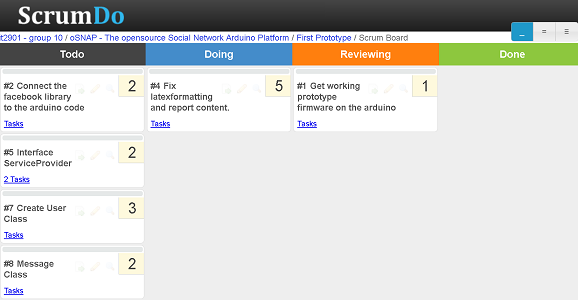
\includegraphics{img/management-scrumdo} \caption{The Scrum Board in ScrumDo}
\label{fig:management-scrumdo}
\end{figure}


\subsection{Software and hardware development tools}
Various software tools will be used througout the project. These include:
IDEs of choice: NetBeans and Eclipse
Collabaration tools: git, svn, Trac
Pre-existing software: Facebook Android SDK, Android SDK, Twitter4j, Scribe and possibily others

The project task requires various hardware, namely Arduino boards, shields and modules and Android mobiles. Our customer kindly arragend for us so that we can borrow Arduino equipment from the lab. The team will use its own
mobiles for running, testing and prototyping the system.
	
Another part of the project is the collaboration software.
Initially we decided to use Git which is a fast, scalable,
distributed revision control system with an unusually rich command
set that provides both high-level operations and full access to internals.
It differs from the centralised control systems like SVN for its capability
to handle several software \char`\"{}branches\char`\"{} at once. The
branches can head in different directions and can later be merged
instead of always maintaing a central, \char`\"{}correct\char`\"{}
version. NTNU provided SVN and Trac repositories to keep track of our
project and we will use these to share finished code for evaluation
purposes. We decided to use Git due to its higher flexibility and because
of the experiences the team members already had with it.

\newpage
\section{Risk analysis and mitigation strategies}

This text will highlight different realistic risks that may occur during development
that can to some degree jeopardise the process or the final product.
A table with weighted risks and relative mitigation and remedial actions follows.

\subsection{Dropouts}
The risk of people dropping the course or otherwise not being able to complete it as part
of the group. This can be caused by sickness as well.

\subsection{Arduino hardware}
Our handed out Arduino equipment can fail, due to malfunctioning or wrong usage.
There is also the possibility that some of the hardware can be lost while we work with it at home.

\subsection{Deadlines}
Throughout the course there is multiple deadlines that must be met. Failure to meet
these limits will have huge impacts on the grading and could possibly fail the group.

\subsection{Choosing wrong frameworks}
We will necessarily have to build parts of our software around existing open source
frameworks to limit effort required by the task. If at a later point we have severe limitations
on our possibilities due to these frameworks the product could result poorer in features than
we originally planned. The impact can be negligible if other solutions are found.

\subsection{Design problems}
During development features have to be constrained due to problems or resource limitations.
This will in turn will cause the final product to not satisfy the customer. If we can find work-arounds
and compromises can be found, then the problem will not have as huge of an impact.

\subsection{Wireless connectivity}
If the Arduino chip modules (called shields) for Bluetooth etc. are too hard to implement
we would have to reconsider wireless connectivity as an option.
We set the 'get wireless to work' deadline to be one month. If we can't get it working
by that time we will have to use cabled connections instead and that would result clumsy
for a lot of concepts.

\begin{table}
	\begin{center}
		\begin{tabular}{| l | l | l | l | p{2.8cm} | p{2.8cm} |}
\hline

Description & Likelihood & Impact & Risk & Mitigation & Remidial Action\\ \hline

Sickness 			& Med & Low & Med & Keep contagious sicknesses at home.
					& If the sickness is prolonged work tasks must be re-arranged appropriately. \\

Wireless Connect. & Low & High & Med & Get it working & Switch to cable connection \\

Arduino Malfun. & Low & Med & Low & Treat hardware properly. Do not eat or drink nearby.
					&  Get new hardware if possible.\\

Lost Hardware & Low & Med & Low & Have control over who has what and keep an inventory list.
					& Get new hardware if possible \\

Limited Product & Low & Med & Low & Thorough planning. Avoid late features implementation.
					&  Workaround problems at critical junctions in the process.\\

API Trouble & Med & Med & High & Limit the scope to documented open source APIs.
			& Investigate alternative solutions. Limit impact on productivity. \\

Final Deadline & Low & High & Med & Consistent work throughout the semester. Avoid last-minute feature implementation.
			&  Deliver the product in the best state possible.\\
Mid-Sem Deadline & Low & High & Med & Produce good documentation and begin early on reports.
			&  Consult with student assistants.\\
		\hline
		\end{tabular}
	\end{center}
	\caption{Risk Analysis}
	\label{table:riskanalysis}
\end{table}

Concluding, most care should be put in the choice of existing frameworks and in early planning
and documentation efforts to avoid later problems related to the implementation and report delivery.

\newpage
\section{Resources}
A meeting table was arranged during the first meeting. Team members
have weekly meetings on Monday, Wednesday and Friday at twelve o'clock.
Meetings with the client were arranged for each Friday at two fifteen.

The team exchanged both e-mails and mobile numbers. A permanent Skype
group chat on which we meet on a daily basis was set up, a mailing
list was also created. Several documents of interest to the group
were made available to everyone using Google Documents.

\todo
{
 Finish these sections.. they are very related
}
20 hours work per person each week.
7 persons
7 * 20 = 140 hours per week
17 weeks * 140 hours = 2380 hours

\subsection{Work Breakdown Structure}


\subsection{Gannt Diagram}



\cleardoublepage
\chapter{Prestudies}\label{ch:prestudies}

This chapter describes the studies made on existing similar solutions,
and the prototype concepts we took into consideration in the early stages of the project.
The customer didn't request a specific prototype; we came up with different ideas and mentioned
them to the customer, until a suitable prototype was agreed on.

\section{Existing solutions}
We did some research on the Internet about similar and related products. It is important to underline that our task was
not just to create another prototype, but instead a set of libraries that would ease future development of new protoypes
connecting Arduino to social networks. These existing products were relevant in order to confirm that tangible user interfaces
for social networks using Arduino were a reality. They also provided some ideas to take into consideration.

\newpage

\subsection{LikeLight}
This product found on the internet (\ref{link:likelight}) is a Facebook like indicator that glows when some content the
user posted on Facebook is liked by someone. It was realized with an Arduino board inside a giant Lego hand.
(Figure \ref{fig:prestudies-likehand})

\begin{figure}[h!]
\centering 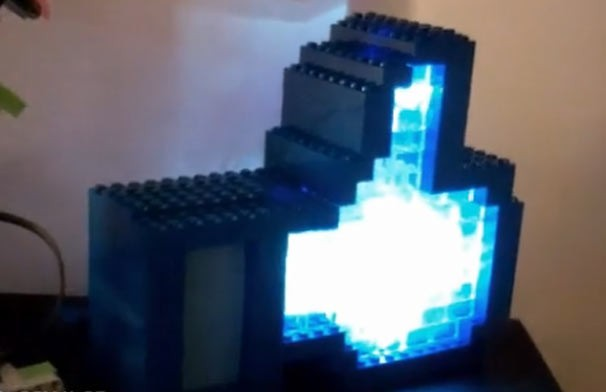
\includegraphics[scale=0.85]{img/prestudies-likehand}
\caption{LikeLight from Red Pepper Labs\cite{link:likelight}}
\label{fig:prestudies-likehand}
\end{figure}

\newpage

\section{Our own ideas}

\subsection{YepMailbox}
The YepMailbox (Figure \ref{fig:prestudies-YepMailbox}) was another concept that we thought of, of a tangible Arduino-powered prototype 
that would interact with the user Facebook wall. The mail flag would rise powered by a small servo motor and a printer 
would print out the new message.

\begin{figure}[h!]
\centering 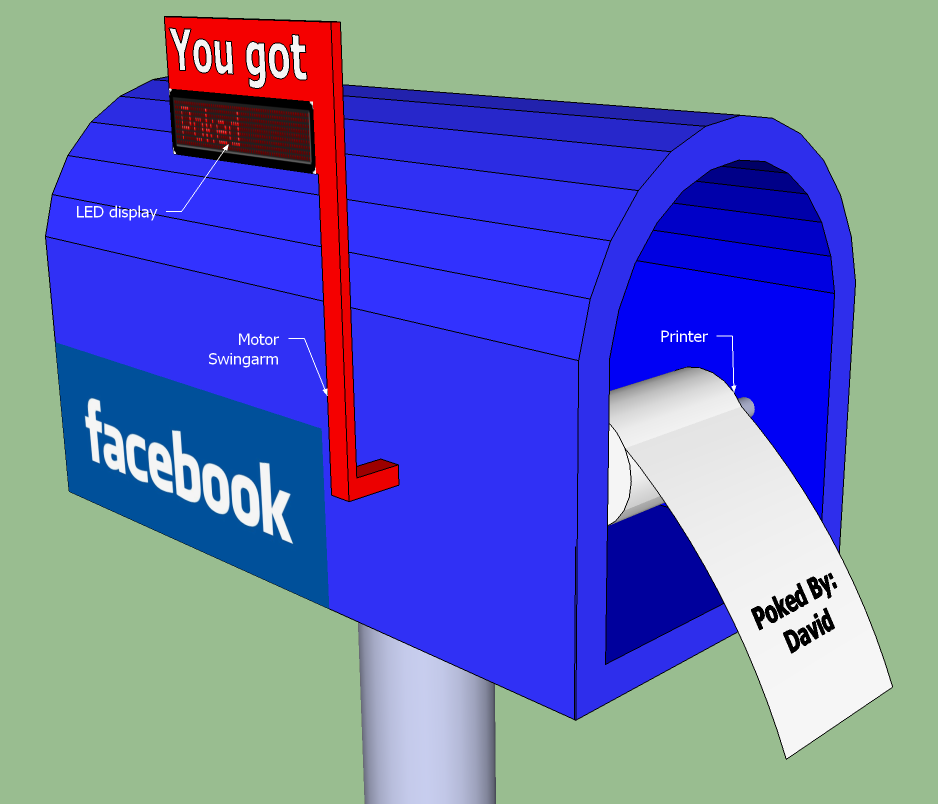
\includegraphics[scale=0.4]{img/prestudies-YepMailbox}
\caption{Our concept idea of the YepMailbox}
\label{fig:prestudies-YepMailbox}
\end{figure}

\newpage

\subsection{Facebook Wall}
The "Facebook Wall" (Figure \ref{fig:prestudies-facebookwall}) is another concept we came up with. It is a wall with two holes in it for people to put their faces in.
The prototype would then make a picture and replace the wall with some image and add bodies to the two faces. The image 
would then be automatically uploaded and posted on Facebook.

\begin{figure}[h!]
\centering 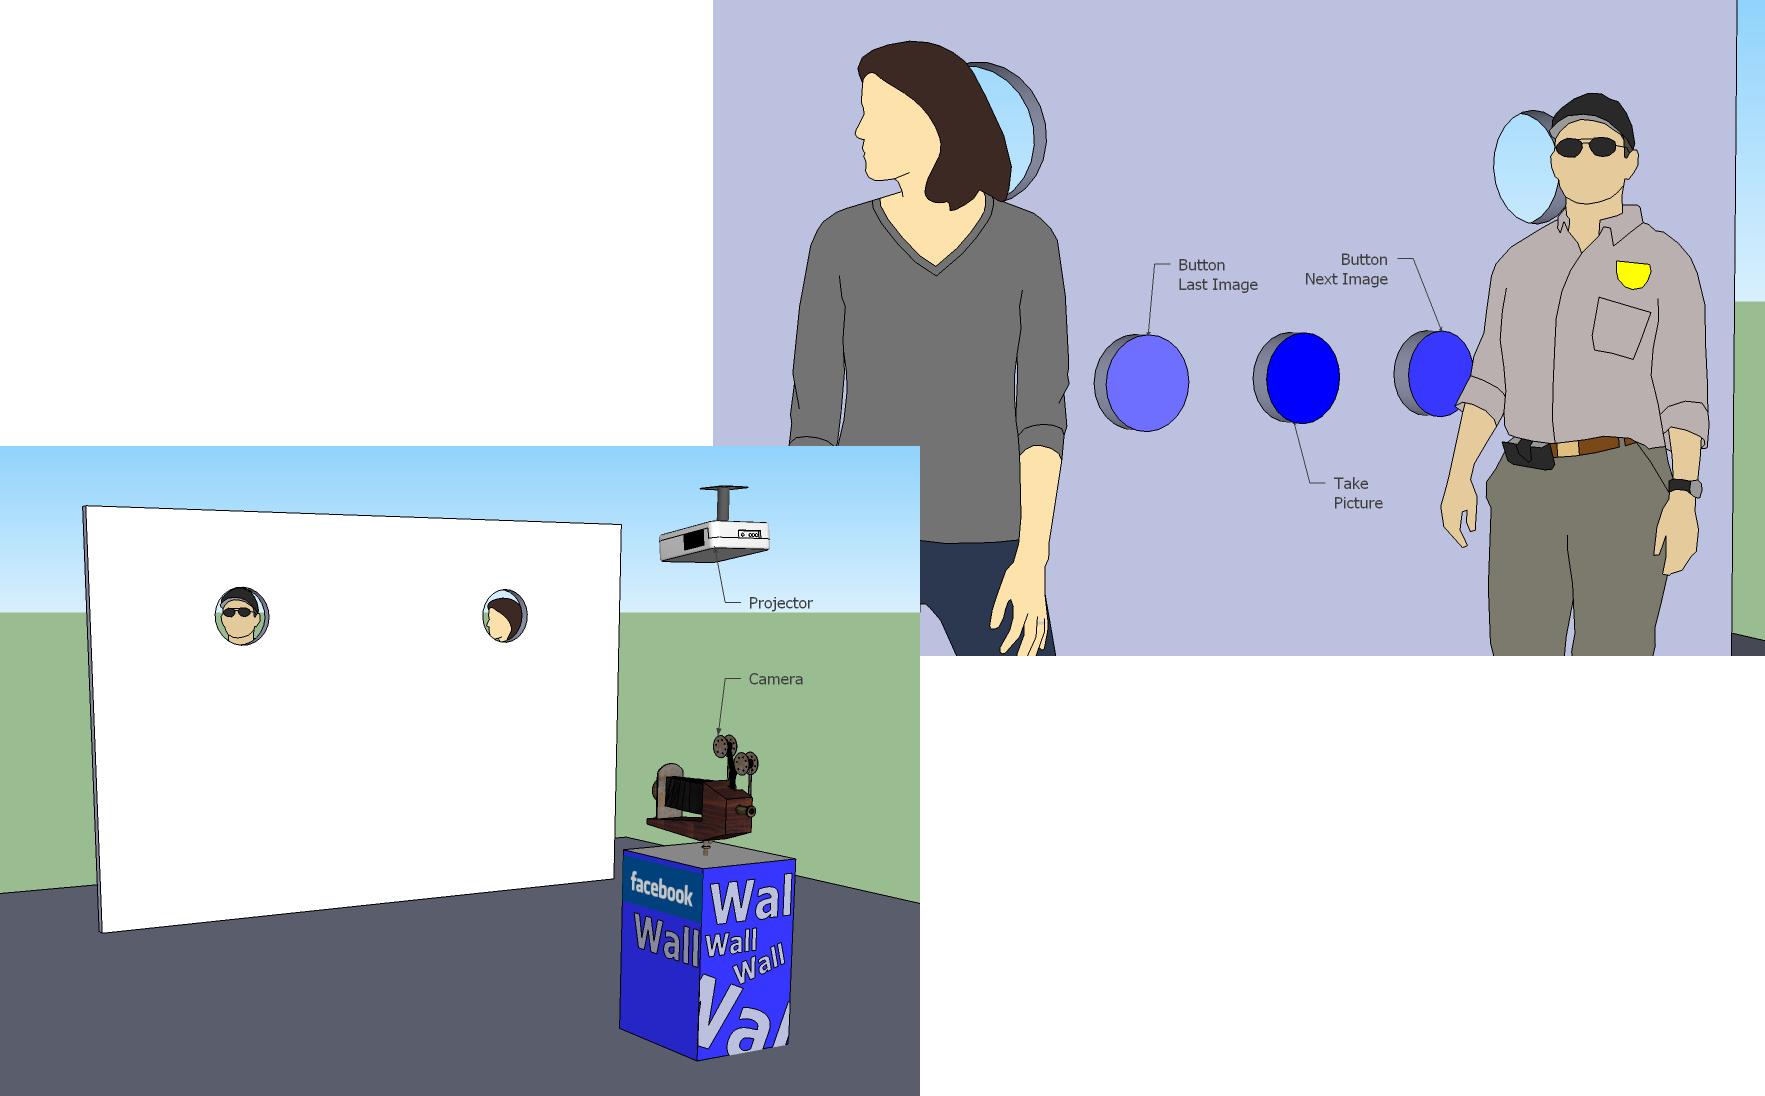
\includegraphics[scale=0.22]{img/prestudies-facebookwall}
\caption{Our concept idea of the Facebook Wall}
\label{fig:prestudies-facebookwall}
\end{figure}

\newpage

\subsection{T-Shirt}
The T-Shirt (Figure \ref{fig:prestudies-tshirt})  features electronic circuits powered by an Arduino Lilypad board.
The Lilypad is an Arduino board designed specifically to be worn. It is connected wirelessly to the Internet through
an Android phone, and downloads status updates from a social network such as Facebook.
The content fetched is then displayed through one of the electronic devices: LEDs, LCD screen,
sound module or a vibration module.


\begin{figure}[h!]
\centering 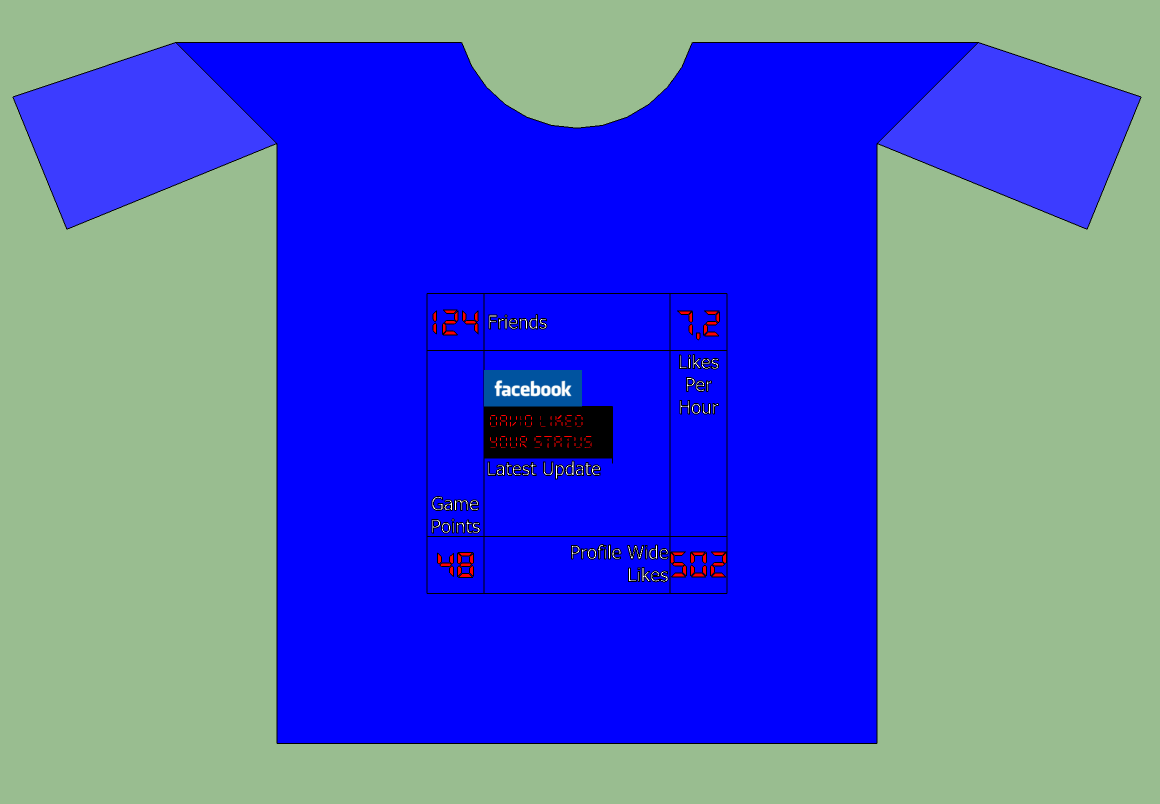
\includegraphics[scale=0.35]{img/prestudies-tshirt}
\caption{Our first concept idea of the T-shirt prototype}
\label{fig:prestudies-tshirt}
\end{figure}

\newpage

\section{Conclusion}
We presented our various ideas and concepts to the customer and let him decide on what he would
like the group to work on. The client liked the t-shirt idea, and he decided that it would be the main prototype for this project. 
After some iterations the t-shirt got swapped out with a jacket due to practical reasons for implementing the hardware. 
The prototypes work as proof-of-concept that our developer libraries function as they should and work as the same time as an 
example on how the libraries can be used. In our example we show how you can connect social networks (Twitter, Facebook, etc.) to 
tangible Arduino interfaces (LED, buzzer, sound, buttons, etc.). The customer requested one or two additional smaller prototypes in 
addition to the oSNAP Jacket to prove that our libraries can be successfully used to develop different prototypes. Each of the prototypes are 
described in more detail in section \ref{sec:prototypes}.


\cleardoublepage
\chapter{Requirements}\label{ch:requirements}

This chapter describes both the functional and non-functional requirements
for the various parts of the project.

\section{Functional requirements}

\begin{table}
		\caption{Requirements}
\begin{tabular}{ | l | c | }
	\hline                        
	\bf{Requirement} & \bf{Priority} \\
	\hline
	F1:  SocialLib					& Very High \\
	F2:  ComLib						& Very High \\
	F7:  T-Shirt Prototype			& High \\
	F3:  oSNAP application			& Medium \\
	F4:  T-Shirt application		& Medium \\
	F5:  Facebook application		& Medium \\
	F6:  Twitter application		& Medium \\
	F8:  Temperature application 	& Low \\
	F9:  Temperature Prototype		& Low \\
	F10: LED matrix application		& Low \\
	F11: LED matrix Prototype		& Low \\
	\hline  
\end{tabular}
\end{table}

\subsection{F1: Social library}
\begin{description}
	\item[Network support:] The library shall support at least two social
	networks. One shall be Facebook.
	\item[Abstractions:] The library shall provide abstractions for concepts
	found in social networks, and simplify Android's IPC mechanisms
	between social services and TUI prototypes applications.
\end{description}
	
\subsection{F2: Communication library}
\begin{description}
	\item[Wireless connectivity:] Since the product will target a user-base
	with no technical background, the customer required all connections
	between devices to be wireless, so that connecting the User Interface
	to the Android mobile will be as easy as possible for the end-users.
	For this reason, the technical details of the connection should be
	hidden to the end-user so that the product can be easily operated.
	\item[Two-way communication:] The communication shall be two-way:
	from the Arduino device to Android and vice-versa.
\end{description}

\newpage

\subsection{F3: oSNAP application}
\begin{description}
	\item[Libraries:] The application shall use the Communication library
	to communicate with TUI prototypes.
\end{description}

\subsection{F4: T-Shirt application}
\begin{description}
	\item[On and Off:] The user shall be able to turn the application On
	and Off. When the application is not running, no social data will be
	forwarded to the T-Shirt prototype.
	\item[Libraries:] The application shall use the Communication library to
	communicate with the T-Shirt prototype and the Social library to
	receive and send data from/to social services.
	\item[Rules:] The application shall let the user setup a set of rules
	to control the behavior of the T-Shirt. Rules can be created and deleted.
	\item[User interaction:] The application shall continue to work
	when the mobile itself is idle.
\end{description}

\subsection{F5: Facebook application}
\begin{description}
	\item[Login (Authentication):] The application shall handle the
	authentication with Facebook.
	\item[Logoff:] The user shall be able to log off once logged in.
	\item[Facebook connectivity:] The application shall fetch and push data
	from/to Facebook as requested, even when the mobile itself is idle
	(not operated).
	\item[Libraries:] The application shall use the Social library to
	communicate with TUI prototype applications.
	\item[User input:] Once the user is authenticated, no further user action
	should be required.
\end{description}

\subsection{F6: Twitter application}
\begin{description}
	\item[Libraries:] The application shall use the Social library to
	communicate with TUI prototype applications.
\end{description}

\subsection{F7: T-Shirt prototype}
\begin{description}
	\item[Features:] The prototype shall map some social content to various
	embedded electronic devices.
	\item[Libraries:] The prototype shall use both the Social and Communication
	libraries.
	\item[User input:] Once the rules for the T-Shirt are set, no further user
	input shall be required.
\end{description}

\subsection{F8: Temperature prototype}
\begin{description}
	\item[Features:] The prototype shall read the temperature using an Arduino
	sensor and send it to Facebook.
	\item[Libraries:] The prototype shall use both the Social and Communication
	libraries.
\end{description}
	
\subsection{F9: LED matrix prototype}
\begin{description}
	\item[Features:] The prototype consists of a matrix of LEDs controlled by an application on 
	an Android smart phone.
	\item[LED Matrix:] The prototype should have a matrix of 3x3 RGB LEDS. Each of the LEDs should be able to display different RGB colour.
	\item[Libraries:] The prototype shall use the Communication library.
\end{description}

\subsection{F10: Temperature application}
\begin{description}
	\item[Mac address:] The user should be able to scan the mac address from a QR code, and/or enter it manually. 
	\item[Share temperature:] The user should have full control over when and to which social media the temperature data is shared.
	\item[Time interval:] The user should be able to set automated updating of the temperature.
	\item[Dependecies:] Facebook service application.
	\item[Libraries:] The application shall use the Social and Communication libraries.
\end{description}

\subsection{F11: BlingLED application}
\begin{description}
	\item[Connection:] You must be able to establish a wireless connection from the Android to the prototype (F9) through Bluetooth.
	\item[Lights:] When the appropiate light levels are adjusted on the Android, the prototype (F9) should adjust the LED matrix accordingly.
	\item[Libraries:] The application shall use the Communication library.
\end{description}

\newpage

\section{Non functional requirements}

\subsection{Libraries}

Both libraries share some non functional requirements.
For the sake of simplicity they will be listed together.

\begin{description}
	\item[Extensibility:] The library shall have a modular design
	in order to be easily extended. The software that will be developed for
	this project will serve as a proof-of-concept and possibly as a starting
	point for other research projects. For this reason a flexible, modular
	software architecture is an important requirement for our customer. The code
	shall be developed in independent, thus reusable modules so that adding new
	functionality will be fairly easy for new developers.
	\item[Target platform:] The library shall be compatible with the Android
	system starting from version 2.2. This will place restrictions on the
	existing software and on the programming languages that will be adopted.
	\item[Documentation:] The library shall be documented using Javadoc.
	Since the product is going to be further developed by other people and is
	mainly designed to simplify application development, a good documentation is
	important. Proper documentation and tutorials should be available to
	third-party developers.
	\item[Licensing:] The library shall be released under the Apache License 2.0
	\footnote{See http://www.apache.org/licenses/LICENSE-2.0.html for more
	information on the Apache 2.0 license}. The customer made clear that all the
	software developed needs to be released under a permissive, Apache software
	license. This implies that pre-existing software that will eventually be
	adopted and incorporated in the project must have a compatible license.
\end{description}

\subsection{Applications}

All the applications share some non functional requirements.
For the sake of simplicity they will be listed below:

\begin{description}
	\item[Target platform:] The applications shall be compatible with the
	Android system starting from version 2.2. This will place restrictions on
	the software and on the programming languages that will be adopted.
	\item[Documentation:] The applications shall be documented using Javadoc.
	\item[Licensing:] The applications and their source code shall be released under the Apache
	License 2.0.
\end{description}


\cleardoublepage
\chapter{Design}\label{ch:architecture}


The whole project encompasses different libraries, prototypes and applications.
This chapter describes the design of each part of the product in detail,
and documents the various approaches taken into consideration.

\section{System overview}

The system consists of:
\begin{description}
	\item[Libraries:] Social library, Communication library
	\item[Applications:] T-Shirt application, other applications
	\item[Prototypes:] T-Shirt prototype, other prototypes
\end{description}

The figure \ref{fig:design-toplevel} illustrates the overall system architecture, demonstration 3 Applications that use only the communication library, only the social service library, or both. Note that in the figure there is no connecion between all the applications and the oSNAP SocialLib. This is intentional because some of the prototypes we will develop will only
use parts of the entire oSNAP library. This is to show that our library is modular and you can use only parts of it and it still works.

\begin{figure}[h!]
	\centering 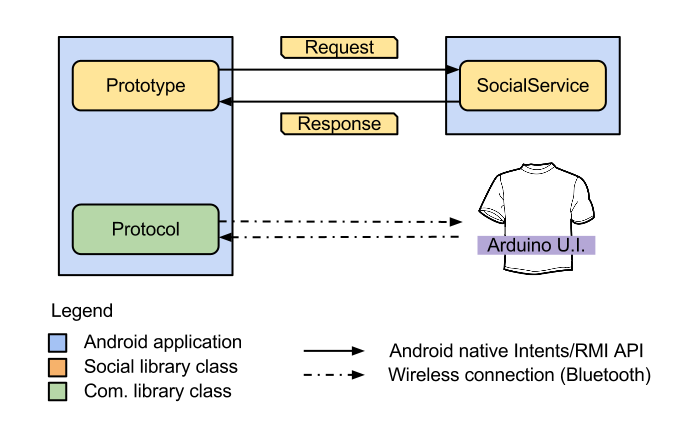
\includegraphics[scale=0.35]{img/design-toplevel.png}
	\caption{Overall system architecture}
	\label{fig:design-toplevel}
\end{figure}


\section{System design}
\label{sec:system-design}
As the requirements for the product were not set early on by the customer, a lot of effort
was put into producing working prototypes to show during the meetings in order to receive
as much feedback as possible and identify the ideas the customer had in mind.
These would provide what was needed to proceed with system design.
At some point thou, after roughly one month, we understood that we were going in the wrong direction,
and that our design wouldn't satisfy the requirements for the use cases the customer mentioned and the
design of some parts of the system had to be revised. It involved especially the Social library and both
the Facebook and T-Shirt applications.

\subsection{First design}
Our first system design was based on the scenario where the user would download the t-shirt
and the social applications, browse for some content from within the social application
and actively send it to the t-shirt application pressing a 'share' button.
This scenario is illustrated in figure \ref{fig:design-usecase1}.

\begin{figure}[h!]
	\centering 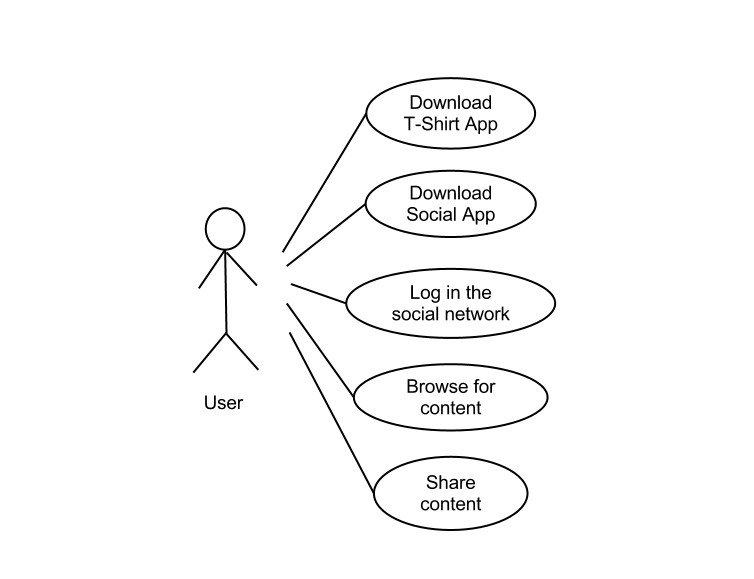
\includegraphics[scale=0.35]{img/design-usecase1}
	\caption{Use case for the product (first design)}
	\label{fig:design-usecase1}
\end{figure}

Please note that in this scenario the user is required to actively send data from
the social application (which acts as a Facebook client) to the T-Shirt application,
which is merely capable of receiving. Also, both are implemented as Android applications.


The figure \ref{fig:design-resp} illustrates the communication between the applications.

\begin{figure}[h!]
	\centering 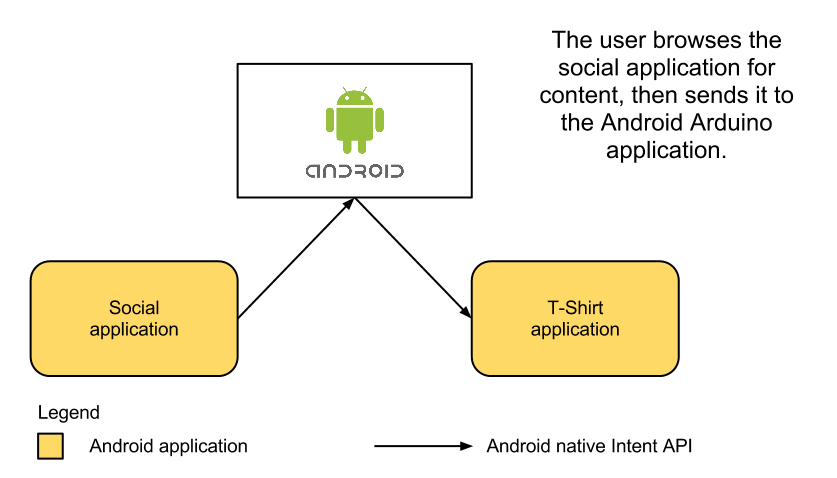
\includegraphics[scale=0.35]{img/design-resp.png}
	\caption{Communication diagram (first design)}
	\label{fig:design-resp}
\end{figure}


\subsection{Second design}
It turned out that the user was not supposed to browse for social content and send it actively
to the T-Shirt application. Instead, after downloading the software, he would just setup a set of rules
specifying the behavior of the T-Shirt. This scenario is illustrated in figure \ref{fig:design-usecase2}

\begin{figure}[h!]
	\centering 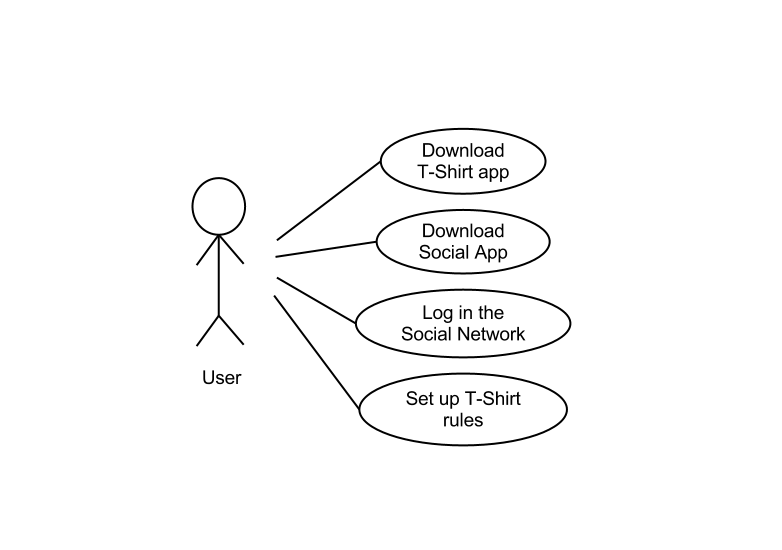
\includegraphics[scale=0.35]{img/design-usecase2}
	\caption{Use case for the product (second design)}
	\label{fig:design-usecase2}
\end{figure}

This new scenario made clear that that both the Social and the T-Shirt applications needed to
be split into:

\begin{itemize}
	\item A user interface, implemented as one or more Android applications, that the user could use to
	authenticate within the social network and setup the rules for the T-Shirt.
	\item Two Android services that would run in the background, without user interaction,
	to fetch data from the social networks and forward it to the Arduino.
\end{itemize}

It also implied that a mechanism to request and exchange social content had to be provided
by the Social library. The figure \ref{fig:design-reqresp} illustrates the communication between
the services and the applications.

\begin{figure}[h!]
	\centering 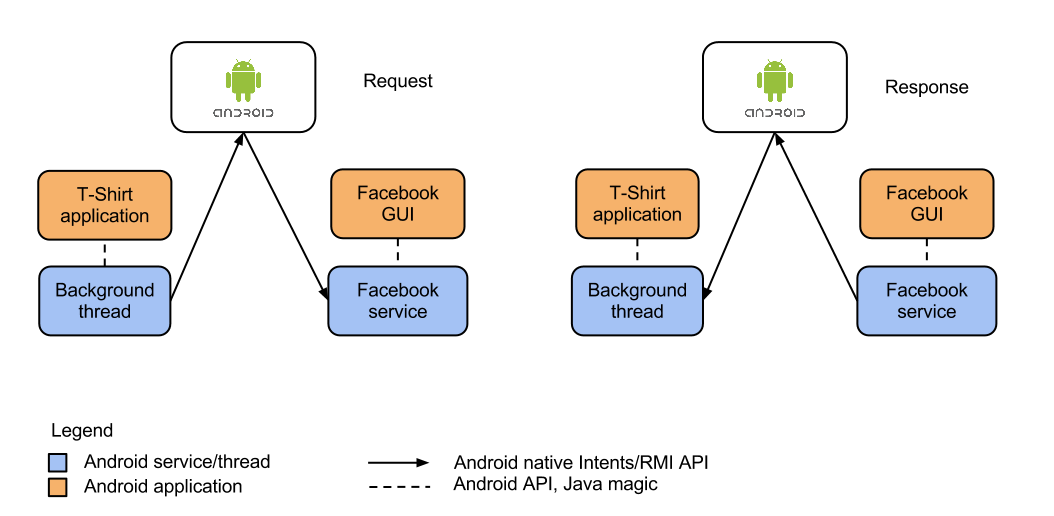
\includegraphics[scale=0.35]{img/design-reqresp.png}
	\caption{Communication diagram (second design)}
	\label{fig:design-reqresp}
\end{figure}

The T-Shirt service is now 'asking' the Social service for a specific content.
This happens in the background, without user interaction.



\subsubsection{Sequence diagram}
This sequence diagram show in figure \ref{fig:design-sequence} shows a sample communication between the Social and T-Shirt applications.
The T-Shirt application requests the list of friends from Facebook whose age is the same as 'Anna'.

\begin{figure}[h!]
	\centering 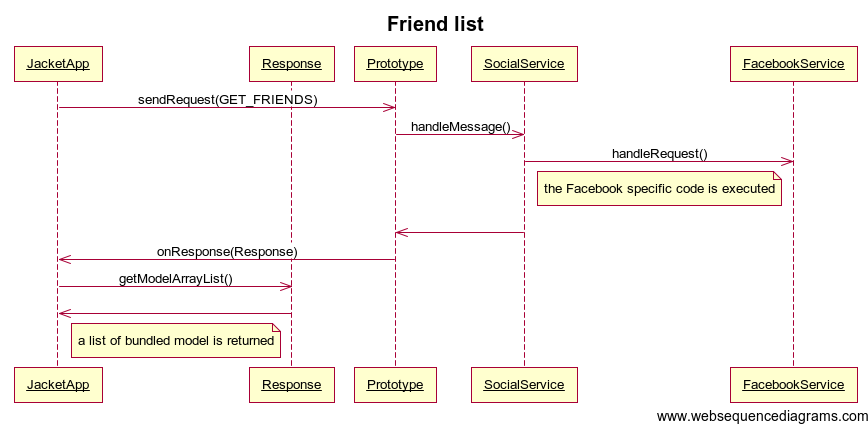
\includegraphics[width=1.0\textwidth]{img/design-sequence.png}
	\caption{Sequence diagram}
	\label{fig:design-sequence}
\end{figure}



\section{Libraries}

\subsection{The social library}
This library provides abstractions for many common concepts found in different
social networks like Facebook or OpenSocial. This is done so that the developers have the possibility
to use these concepts seamlessly between any network and extend them to possibily support others.
It also defines and implements a sort of 'protocol' to allow Android applications and/or services
to exchange social data. This mechanism is based on Android Intent's API.

\subsubsection{First approach}
Our first design approach consisted in a library that would handle the connection to social networks
such as Facebook, Twitter, LinkedIn, etc. This would  allow the developers to write full-fledged
social 'multi-network' clients. It would also provide abstractions for many common concepts
found in these networks such as Post, User, Comment and so on.

\subsubsection{Revised approach}
The big difference in the new approach is that the Social library won't provide any means
of connecting to social networks. Instead it will focus on estabilishing a communication interface,
using Android's Intent mechanism and inter-process communication, between Social applications and
the Android-Arduino applications to allow the requesting and forwarding of social data.
It will still provide abstractions for common concepts found in social networks.
This revised approach was made necessary after the first meetings with the customer as we misunderstood
the project scope, and went on to solve a very ambitious and unneeded task. The new design also accomodated
very well the overall system design. Some of the code and documentation we produced for the previous design
was re-used, but some could not.

\todo{
	a class diagram maybe?
}


\subsection{The communication library}
This library consists of a Java library (implemented on Android) and an Arduino firmware (figure \ref{fig:comlib-diagram}). 
Both implement the ComLib protocol. The Java library provides a set of classes that allow to easily connect to Arduino 
devices that run the Communication library Arduino firmware. The library also implements a mechanism to request a list of 
services the remote device supports and any software download links associated with the remote device. A service might
be a sensor, a lamp, display screen while download links are represented as an URI link. All this meta information is stored
on in the firmware on the remote device as raw text using the JSON format. This metadata can also be stored an retrieved
in a QR code or anything else that can store plain text.

\begin{figure}[h!]
	\centering 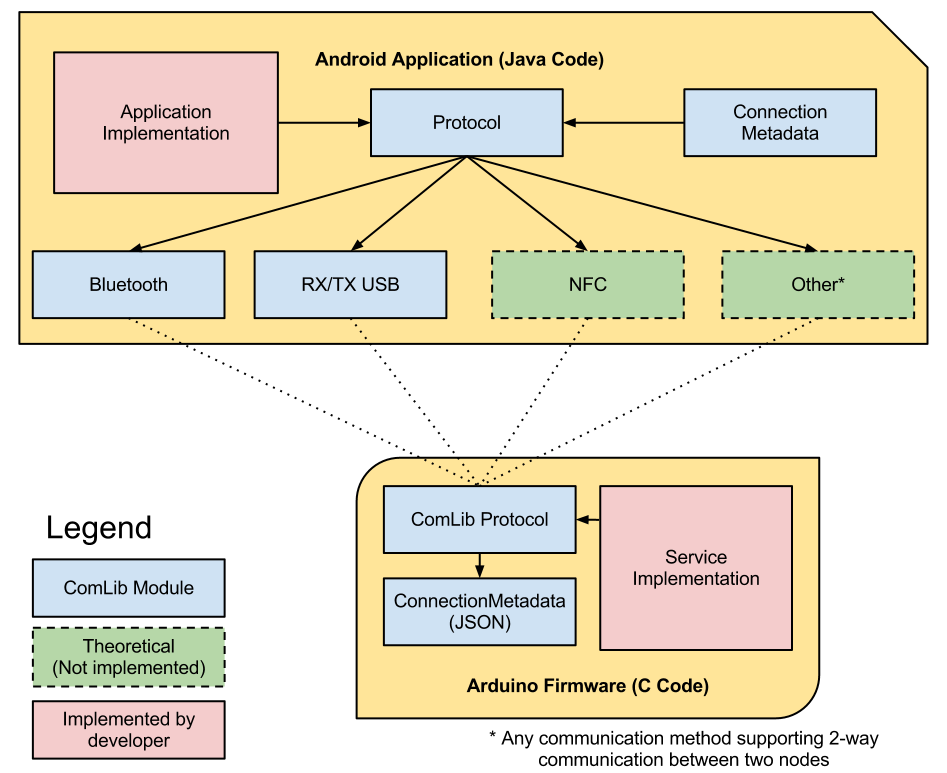
\includegraphics[scale=0.4]{img/comlib-diagram.png}
	\caption{Diagram for the Communication Library design}
	\label{fig:comlib-diagram}
\end{figure}

\subsubsection{The ComLib protocol}
The protocol is a basic set of rules that define how devices can communicate to the Arduino.
The ComLib protocol itself was designed by us, and has seen much changes in terms of which instructions were to be included,
and how the communication was to be executed. With the current design the Arduino cannot initiate the communication,
but is instead a passive device. For all instructions sent by any device to the Arduino, the Arduino sends a response,
either to acknowledge that it is finished executing the corresponding tasks, or the actually return the required
information in the "Content" field. An overview of the current instructions in the protocol can be seen in Table~\ref{tbl:opcodes}.

\begin{table}[h!]
	\begin{tabular}{ | c | c | p{1.5cm} | p{1.7cm} | p{6cm} |}
		\hline
		\textbf{Name} & \textbf{OPCODE} & \textbf{Flag} & \textbf{Content} & \textbf{Description} \\
		\hline
		Ping & 0x00 & N/A & N/A & Pings the arduino, to check that it's there \\
		\hline
		Text & 0x01 & N/A & Text to send & Sends text to the arduino, which then displays it depending on the implementation on the ardunio \\
		\hline
		Sensor & 0x02 & Sensor number & N/A & Requests sensor information from the arduino \\
		\hline
		Pin pulse & 0x03 & Pin number & N/A & Sends a 500ms pulse on the specified pin \\
		\hline
		Pin read & 0x04 & Pin number & N/A & Reads the current digital state of the specified pin on the arduino \\
		\hline
		Pin write & 0x05 & Pin number & Pin value (0~or1) & Writes a digital state of a pin on the arduino \\
		\hline
		Response & 0xFE & Opcode & Response content & A response to a previous instruction, where the flag is the opcode for which it is the response to \\
		\hline
		Reset & 0xFF & N/A & N/A & Resets the arduino \\
		\hline
	\end{tabular}
	\caption{Overview of protocol's instructions}
	\label{tbl:opcodes}
\end{table}

\subsubsection{Arduino firmware implementation}
On the Arduino, all code related to our protocol is abstracted into a ComputerSerial library.
This library is a very basic state machine which processes single bytes received (see Figure~\ref{fig:arduino_states}).
The user of this library can register local methods to be called with RPC when the corresponding instruction is called.
The instructions follow strict rules on how they are constructed (see Table~\ref{tbl:instr_struct} for sizes of the different parts).
Each instruction has to start with a "start-byte" which is always 0xFF. The next part is the size, which tells the number of bytes
to come for this instruction (including the size byte itself). The rest is defined from which instruction is sent, but it is important to
remember that the content cannot be empty, and has to at least contain 1 byte. This byte however, is not necessarily read or used.

The following figure illustrates the Arduino automata.

\begin{figure}[h!]
	\centering
	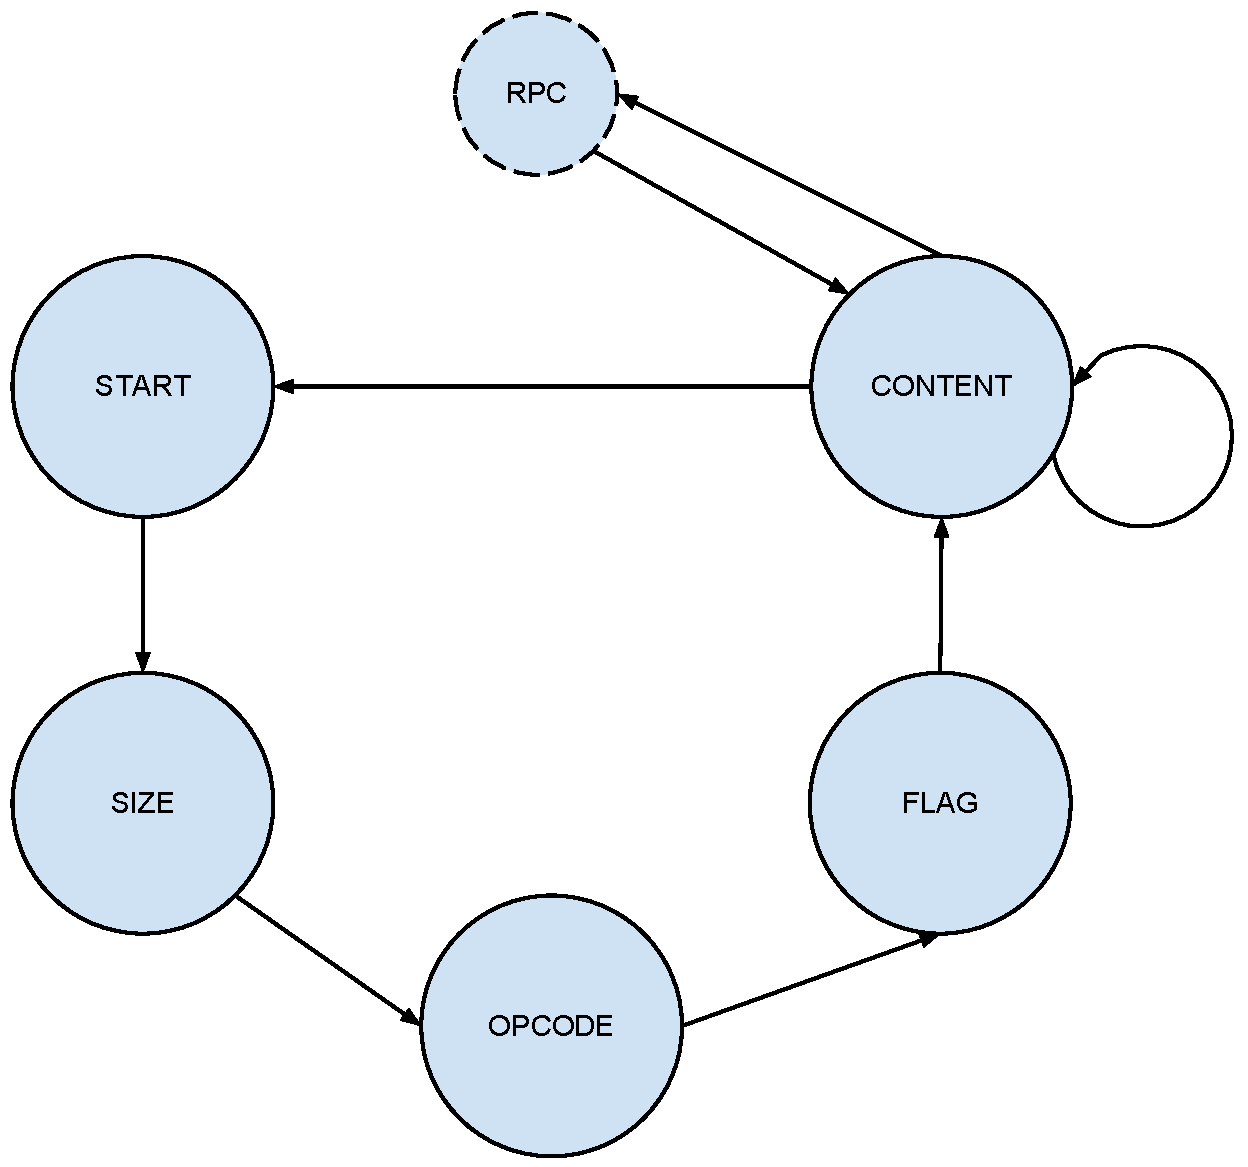
\includegraphics[width=\textwidth, keepaspectratio]{img/arduino_state-machine.pdf}
	\caption{The Arduino state-machine}
	\label{fig:arduino_states}
\end{figure}

\begin{table}
	\begin{tabular}{c|c|c|c|c|c|}
		\cline{2-6}
		& \textbf{Start-byte} & \textbf{Size} & \textbf{Opcode} & \textbf{Flag} & \textbf{Content} \\
		\hline
		\multicolumn{1}{|c|}{\textbf{Size}} & 1 & 1 & 1 & 1 & 1-252 \\
		\hline
	\end{tabular}
	\caption{Byte-structure of instructions}
	\label{tbl:instr_struct}
\end{table}


\section{Applications and Services}

\subsection{T-Shirt application}

As discussed in chapter \ref{sec:system-design} the T-Shirt application design had to be reviewed after roughly one month.

\begin{figure}[h!]
	\centering 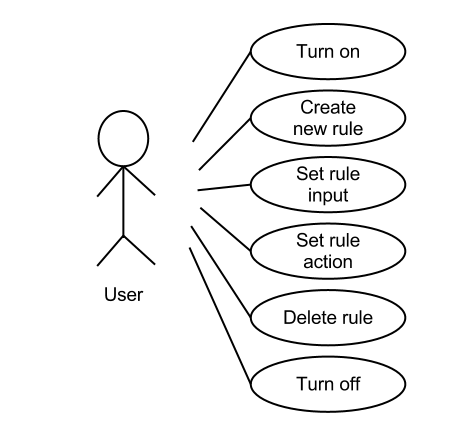
\includegraphics[scale=0.35]{img/design-tshirtappusecase2}
	\caption{Use case for the T-Shirt application}
	\label{fig:design-tshirtappusecase2}
\end{figure}

For completeness we present the previous application use case in figure \ref{fig:design-tshirtappusecase1}

\begin{figure}[h!]
	\centering 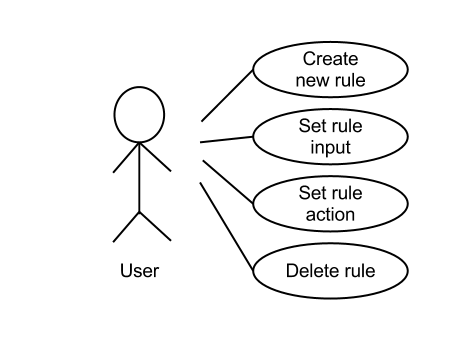
\includegraphics[scale=0.35]{img/design-tshirtappusecase1}
	\caption{Initial use case for the T-Shirt application}
	\label{fig:design-tshirtappusecase1}
\end{figure}

\subsection{Facebook application}

As discussed in chapter \ref{sec:system-design} the Facebook application design had to be reviewed after roughly one month.

\begin{figure}[h!]
	\centering 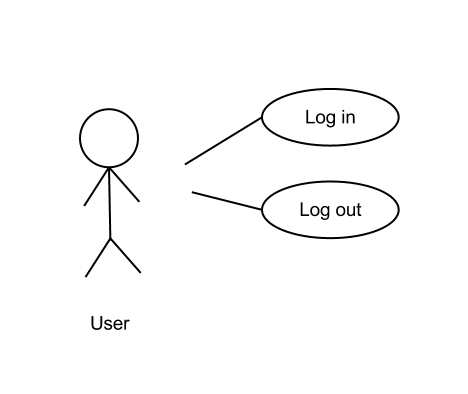
\includegraphics[scale=0.35]{img/design-socialappusecase2}
	\caption{Use case for the Social application}
	\label{fig:design-socialappusecase2}
\end{figure}

For completeness we present the previous application use case in figure \ref{fig:design-socialappusecase1}.

\begin{figure}[h!]
	\centering 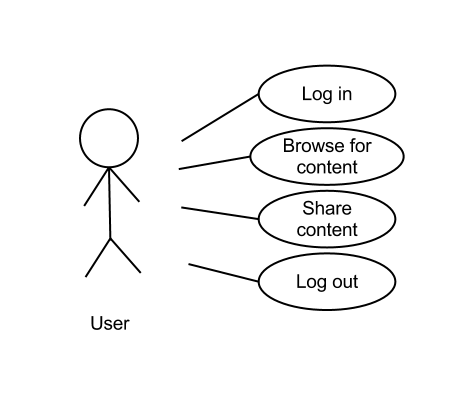
\includegraphics[scale=0.35]{img/design-socialappusecase1}
	\caption{Initial use case for the Social application}
	\label{fig:design-socialappusecase1}
\end{figure}



\section{Prototypes}
\label{sec:prototypes}
Three different prototypes will be produced for the project. They serve both as a proof of concept and
to test that the library works. Each of the prototypes should be different to show that the library can be
used to quickly prototype Arduino Tangible User Interfaces. One of the protoypes, the T-Shirt, is significantly
bigger and more complex than the other two. The T-Shirt is the main prototype of the project; the purpose of the other two
is just to show that the libraries can be use for other applications and in different contexts.

\subsection{Prototype 1: The social T-Shirt}
	
\begin{figure}
	\begin{center}
	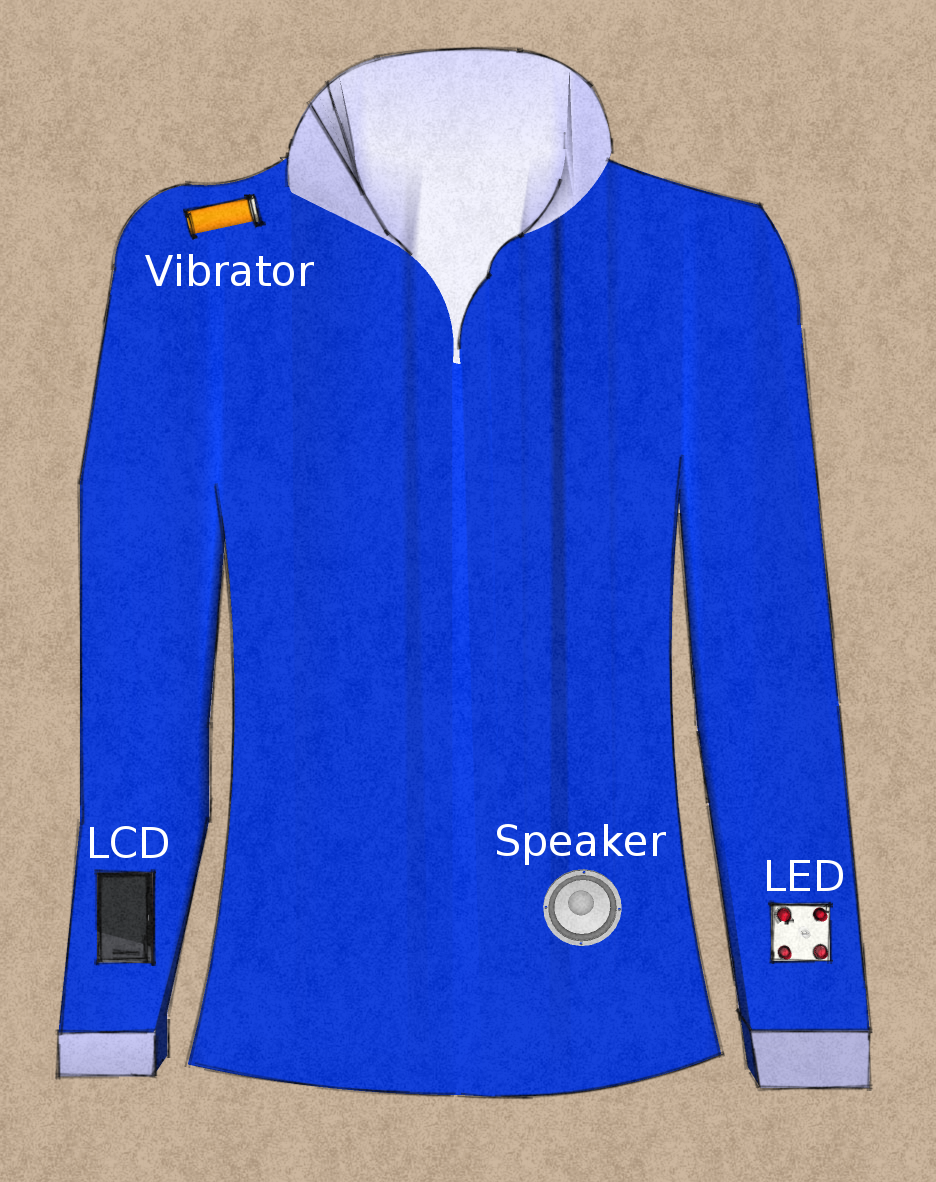
\includegraphics[scale=0.2]{img/design-tshirtproto}
	\end{center}
	\caption{Concept drawing of the T-Shirt Prototype}
	\label{fig:design-TShirt}
\end{figure}
	
This is our main prototype and will showcase a lot features.
It consists of a T-Shirt or sweater connected to a Lilypad Arduino that will feature
several displays and indicators which will receive social data from the Android phone.
The shirt features different tangible interfaces (see figure \ref{fig:design-TShirt}):
	
\begin{itemize}
	\item LEDs
	\item LCD Display
	\item Sound speaker
	\item Vibration module
\end{itemize}
	
Any of these can be mapped to a fair deal of concepts found in social network.
So a "Poke" from Facebook could become a vibration on the T-Shirt. When someone "Likes" your post a small sound effect
could be played, a LED blinking on status updates from Twitter, etc. The T-Shirt is connected to the social networks
throu a wireless connection to the Android mobile. Specifically, the mobile Android is connected to the internet
and carried in the pocket of the person using the T-Shirt and is connected wirelessly with the Arduino Lilypad through Bluetooth.
	
	%\begin{figure}[h!]
	%\centering 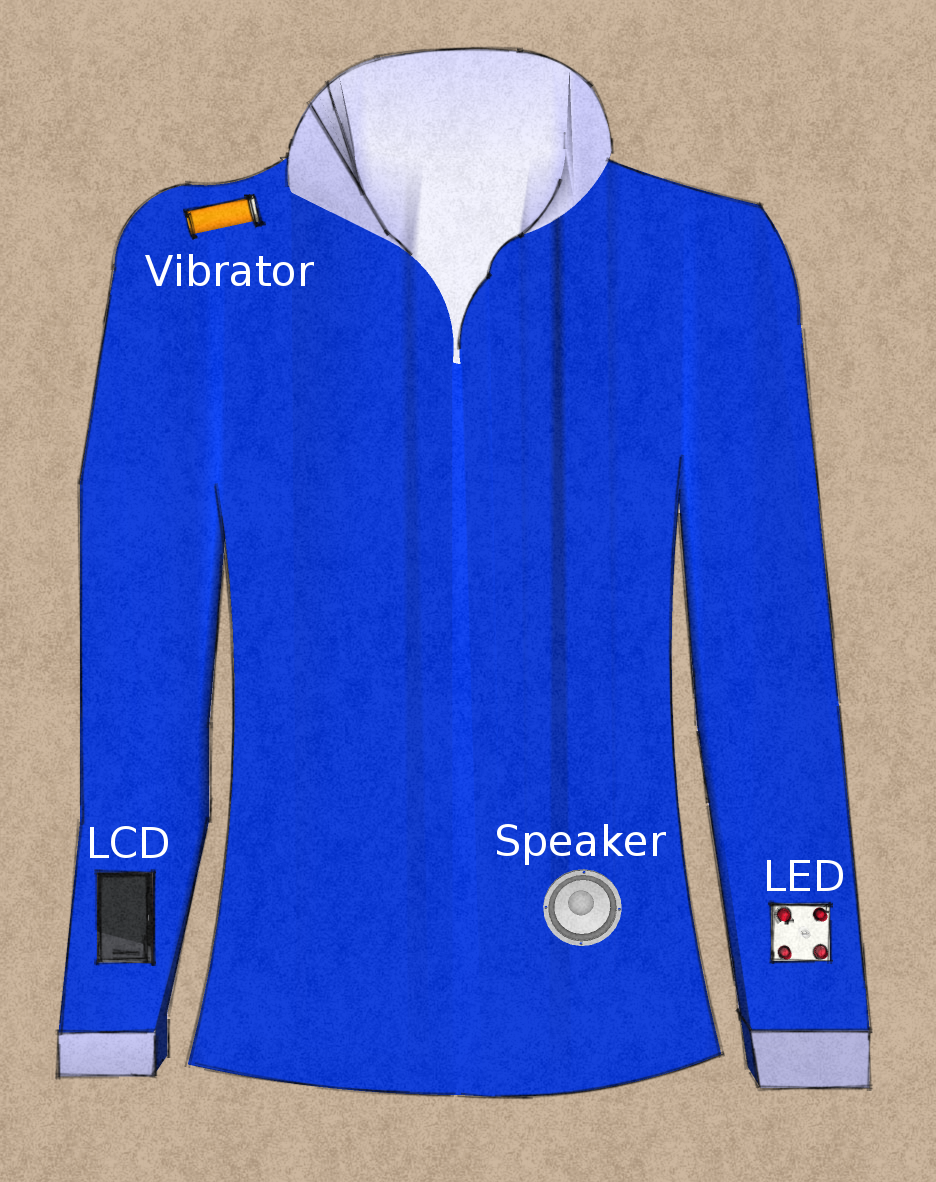
\includegraphics[width=1.0\textwidth]{img/testing-tshirtproto}
	%\caption{Concept drawing of the T-Shirt Prototype}
	%\label{fig:testing-TShirt}
	%\end{figure}


	
\subsection{Prototype 2: Temperature Sensor for Android}
This prototype will primarily showcase the communication from Arduino to Android using our libraries.
A temperature sensor will be connected to an Arduino board and then constantly send its output over bluetooth to a
an Android application. Figure \ref{fig:design-temperature} shows a visual representation of the entire Temperature Sensor
prototype with an Android device connected wirelessly through bluetooth to the Arduino board.

\begin{figure}
	\begin{center}
	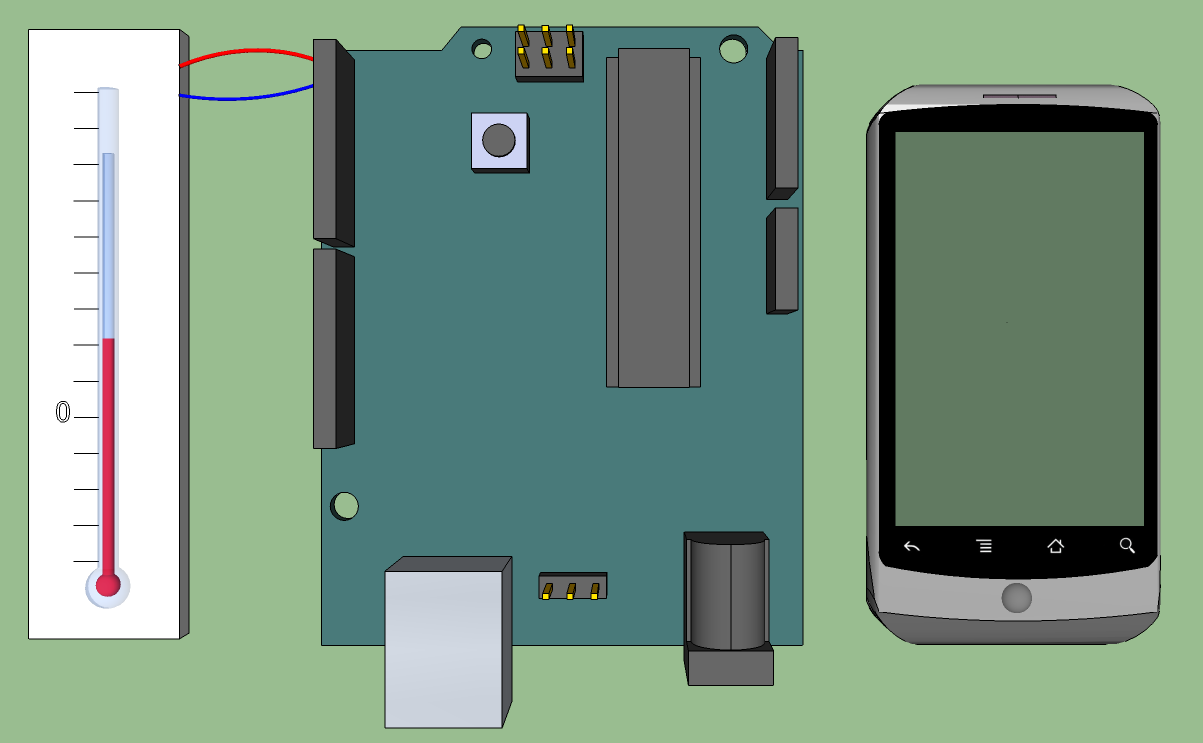
\includegraphics[scale=0.35]{img/design-temperature}
	\end{center}
	\caption{Concept drawing of the temperature application setup.}
	\label{fig:design-temperature}
\end{figure}

\subsection{Prototype 3: Wearable Pictures}
This prototype was first planned to be LED lights (Figure \ref{fig:design-ledmatrix}) showing what mood you had on MySpace. Red LED lights would be angry,
green would be happy and so on. We discovered that MySpace had removed this feature from their pages, even if it was
still supported by the API. It would be a fools errand to pursue something you could not test properly
in a real world situation, so we changed the concept of this prototype. It ended up to be a sort of wearable fashion.
The user can take a picture or choose one on his Android mobile and send it to the prototype Android application.
The picture is then sent with an Intent using the Android API, making it easy to start our program and receive
the bundled picture. For prototyping purposes the wearable product will feature just a few LEDs which our Android
prototype program will map to certain pixels and then transmit over Bluetooth to the Arduino
component and this will promptly light the LEDs.

\begin{figure}
	\begin{center}
	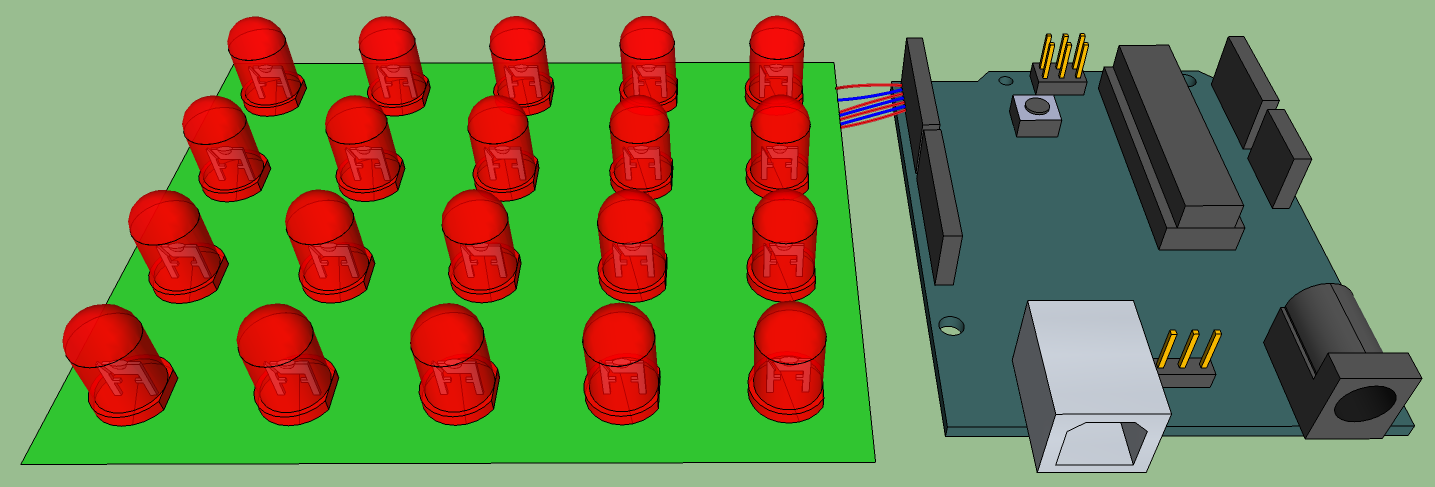
\includegraphics[scale=0.35]{img/design-ledmatrix}
	\end{center}
	\caption{Concept matrix of LED to show simple image.}
	\label{fig:design-ledmatrix}
\end{figure}

\section{Package Structure}
The system can be divided into smaller sections. This section describes some of the structures
we have divided the system into. The most obvious distinction is between the Java code runs
on the Android platform and the C code which is executed by the Arduino platform.
The Java code is again divided into packaged libraries as described below.

\subsection{Java code}
\begin{itemize}
	\item \textbf{no.ntnu.osnap.com}\newline
		Communication Library contains every class to establish a connection with a remote device using a general
		protocol interface. The actual details of the communication such as Bluetooth, cable, WiFi, stream-based or
		sockets are hidden away from the user. This is to provide a simple and generic interface to all supported
		communication methods. The user can easily add new communication types by extending an abstract class.
		The ComLib additionaly defines a standard of storing and retrieving metadata of services and download URI
		links from the remote device using JSON.
	\item \textbf{no.ntnu.osnap.com.testing}\newline
		Test units and sample programs for the ComLib. These are simple test applications that are run on
		the Android to test if the ComLib is communication correctly using the specified
		protocol.
	\item \textbf{no.ntnu.osnap.social}\newline
		Social Library provides an easy to use interface between social services and applications/services
		running on the Android platform. The SocialLib also provides some general data models such as Person,
		Group or Message for concepts commonly used in most social networks. 
	\item \textbf{no.ntnu.osnap.social.testing}  \newline
		Test units and sample programs for the SocialLib.
\end{itemize}

\subsection{Arduino C code}
All the arduino code is in one class, and there is therefore no package structure to speak of. The class consists of a header file and a source file. This is then to be included in arduino projects that want to use our protocol for communication.



\cleardoublepage
\chapter{Sprints}\label{ch:sprints}

This chapter describes the work done in each sprint. A sprint is one iteration
of the Scrum process (see section \ref{section:scrum} for more information about
Scrum). The duration of each sprint was two weeks. Every sprint was assigned
various tasks from the project backlog. Task IDs were assigned to task as they
were created. Each task was given a specific point value and assigned to one or
more team members. The point value is an estimation of the amount of work
(measured in man-hours) that is required to complete the task. The point value
can be also influenced by the importance of the task. If a task required more
time than planned and was not finished by the end of the sprint, it was assigned
a 'prolonged' status and moved to the next sprint.

For table layout reasons we used some name abbreviations for the names
of the members assigned to the task.

\begin{table}[ht!]
\begin{tabular}{ | c | l | }

\hline
\textbf{Abbreviation} & \textbf{Name} \\
\hline

 AN & \anders	\\
\hline
 AS & \asbjorn	\\
\hline
 B  & \bjornar	\\
\hline
 E  & \emanuele	\\
\hline
 JH & \johan	\\
\hline
 JN & \jonas	\\
\hline
 H  & \henrik	\\
\hline

\end{tabular}
\end{table}

\newpage

\section{Sprint 1}

Duration: 20/01 to 02/02\newline
Points total: 89

The first sprint was dedicated to planning meetings and working hours
and studying about interested technologies. While some team members had some
experience with Arduino, none of us had any experience with Android application
development and social networks. Each member chose his own role in the project,
based on his own area of interest. The team did a lot of brainstorming in
order to identify possible product ideas to show the customer and produced a
small proof-of-concept application to show during the first meeting with the
customer, which was arranged for the beginning of the second week.

\begin{table}[ht!]
\begin{tabular}{ | r | l | c | c | r | }

\hline
\textbf{ID} & \textbf{Task} & \textbf{Points} & \textbf{Assigned to} & \textbf{Status} \\
\hline

 7 & Brainstorm ideas about the product		& 18 & Everyone		& done \\
\hline
 8 & Search for similar products			& 14 & Everyone		& done \\
\hline
 9 & Proof-of-concept application			& 12 & AN,B,E,JH	& done \\
\hline
11 & Read on OpenSocial						& 10 & E,H,JN		& done \\
\hline
13 & Read Facebook developers' pages		& 10  & E			& done\\
\hline
12 & Read on Arduino						& 8  & AN,AS,B,JH	& done \\
\hline
10 & Choose a development process			& 6  & Everyone		& done \\
\hline
 6 & Meet with the customer					& 4  & Everyone		& done \\
\hline
 2 & Plan group meetings					& 2  & Everyone		& done \\
\hline
 5 & Plan meetings with the customer		& 2  & Everyone		& done \\
\hline
 1 & Exchange contact information			& 1  & Everyone		& done \\
\hline
 4 & Setup mailing list						& 1  & JN			& done \\
\hline
 3 & Setup a Skype chat						& 1  & JH			& done \\
\hline

\end{tabular}
\end{table}

\newpage

\begin{figure}[h!]
\centering 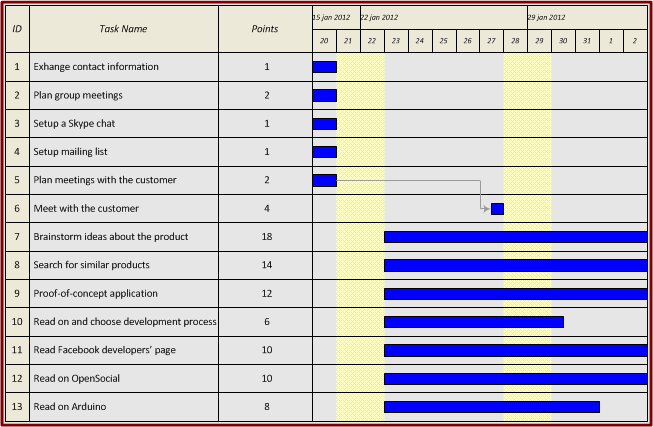
\includegraphics[scale=0.8]{img/sprints-gantt1.png}
\caption{Gantt diagram for the first sprint}
\label{fig:sprints-gantt1}
\end{figure}

\newpage

\section{Sprint 2}

Duration: 03/02 to 16/02\newline
Points total: 96

The second iteration was focused on producing more prototypes of the product to
show the customer in order to receive the necessary feedback to identify
the product requirements and to begin designing the different parts of the
system, as well as acquiring the necessary knowledge and confidence with the
involved technologies. The team also worked on the preliminary version of the
report. The customer suggested that in order to show the re-usability
capabilities of the code, two more prototypes, considerably simpler than the
T-shirt prototype, could be produced for the project.

\begin{table}[ht!]
\begin{tabular}{ | r | l | c | c | r | }

\hline
\textbf{ID} & \textbf{Task} & \textbf{Points} & \textbf{Assigned to} &\textbf{Status} \\
\hline

 2 & Delivery of preliminary report				& 24 & Everyone		& done \\
\hline
 1 & Build a working prototype (week 1)			& 18 & Everyone		& done \\
\hline
 6 & Study Android app. develop.				& 18 & Everyone		& done \\
\hline
 7 & Study Facebook Android SDK					& 12 & E			& done \\
\hline
 3 & Build a working prototype (week 2)			& 8  & Everyone		& done \\
\hline
 4 & Bluetooth connection to Arduino			& 8  & AN,JH		& done \\
\hline
 5 & Connect to Facebook (FB SDK)				& 6  & E			& done \\
\hline
 8 & Setup ScrumDo								& 1  & AN,H			& done \\
\hline
 9 & Setup GIT repository						& 1  & JN			& done \\
\hline

\end{tabular}
\end{table}

\begin{figure}[h!]
\centering 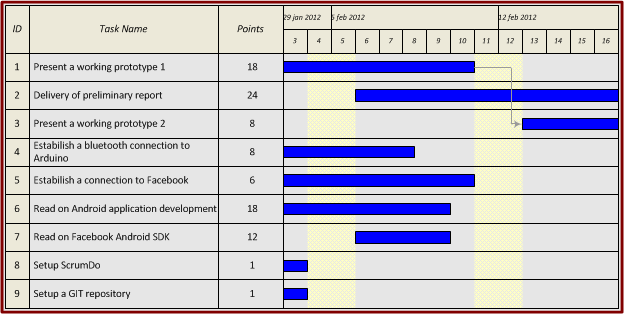
\includegraphics[scale=0.8]{img/sprints-gantt2.png}
\caption{Gantt diagram for the second sprint}
\label{fig:sprints-gantt2}
\end{figure}

\newpage

\section{Sprint 3}

Duration: 17/02 to 01/03\newline
Points total: 108

This sprint was focused on proceeding with the design using the customer
feedback on the prototypes presented so far. An initial version of the
Communication library was also designed and coded. Design of the Social library
also began; various IPC solutions available in an Android system were taken into
consideration. During this sprint the system overall design started to take
shape, and the various parts of the system became more definite. The team
delivered a list of hardware needed to build the various TUI prototypes.
The customer was happy with the team work so far and provided very valuable
feedback.

\begin{table}[ht!]
\begin{tabular}{ | r | l | c | c | r | }

\hline
\textbf{ID} & \textbf{Task} & \textbf{Points} & \textbf{Assigned to} & \textbf{Status} \\
\hline

 4 & Social library design (part 1/2)				& 20 & E		& done \\
\hline
 5 & Comm. library design (part 1/2)				& 20 & AN,JH	& done \\
\hline
 1 & Build a working prototype (week 1)				& 18 & Everyone & done \\
\hline
 6 & Comm. library coding (part 1/3)				& 16 & AN,JH	& done \\
\hline
 3 & Initial system design							& 14 & E,H		& done \\
\hline
 7 & Read on Android IPC mechanisms					& 12 & E		& done \\
\hline
 2 & Build a working prototype (week 2)				& 8 & Everyone	& done \\
\hline

\end{tabular}
\end{table}

\begin{figure}[h!]
\centering 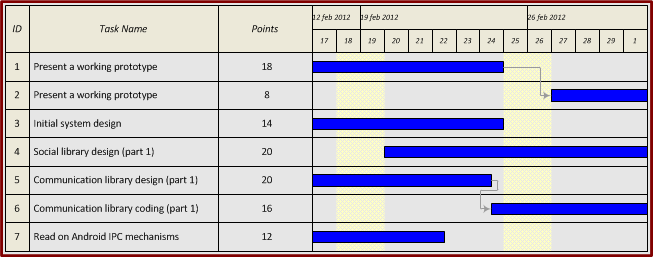
\includegraphics[scale=0.8]{img/sprints-gantt3.png}
\caption{Gantt diagram for the third sprint}
\label{fig:sprints-gantt3}
\end{figure}

\newpage

\section{Sprint 4}

Duration: 02/03 to 15/03\newline
Points total: 112

This sprint was mainly aimed to the delivery of the mid-term report as well
as polishing of the Communication library. The system design proceeded as
planned while the design of the Social library couldn't be completed in time
due to some issues. The team had a hard time trying to find a satisfying
solution. These issues were presented to the customer who provided valuable
feedback that helped solve them.

\begin{table}[ht!]
\begin{tabular}{ | r | l | c | c | r | }

\hline
\textbf{ID} & \textbf{Task} & \textbf{Points} & \textbf{Assigned to} & \textbf{Status} \\
\hline

 1 & Work on the report					& 24 & Everyone & done \\
\hline
 2 & Build a working prototype			& 18 & Everyone & done \\
\hline
 3 & System design						& 18 & E 		& done \\
\hline
 7 & Comm. library coding (part 2/3)	& 16 & AN,JH	& done \\
\hline
 4 & Social libray design (part 2/2)	& 14 & E,H		& prolonged \\
\hline
 6 & Comm. library design (part 2/2)	& 12 & AN,JH	& done \\
\hline
 5 & Social library coding (part 1/3)	& 10 & E 		& done \\
\hline

\end{tabular}
\end{table}

\begin{figure}[h!]
\centering 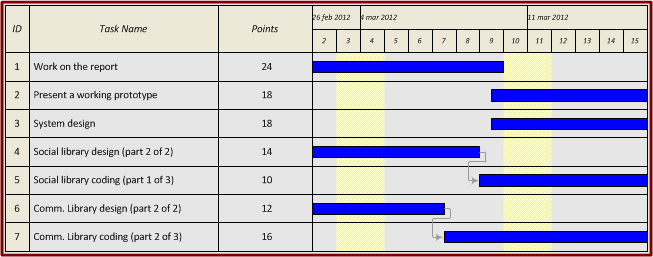
\includegraphics[scale=0.8]{img/sprints-gantt4.png}
\caption{Gantt diagram for the fourth sprint}
\label{fig:sprints-gantt4}
\end{figure}

\newpage

\section{Sprint 5}

Duration: 16/03 to 29/03\newline
Points total: 128

During this sprint the team produced yet another prototype for the customer
and proceeded with the design and coding of the Social library. Coding of the
Communication library also continued, and an initial version was deployed by the
end of the sprint. The team also did some brainstorming and identified the other
two prototypes that were to be presented together with the T-shirt. Some
proof-of-concept applications for these prototypes were also made. This sprint
was a bit more intensive than the previous ones to cope with the fact that the
next sprint would have coincided with Easter vacation. The team still had not
received the hardware needed in order to begin building the T-shirt prototype.

\begin{table}[ht!]
\begin{tabular}{ | r | l | c |c | r | }

\hline
\textbf{ID} & \textbf{Task} & \textbf{Points} & \textbf{Assigned to} & \textbf{Status} \\
\hline

 2 & Social library design (part 2/2)			& 24 & E 		& completed \\
\hline
 4 & Comm. library coding (part 3/3)			& 22 & AN,JH	& done \\
\hline
 3 & Social library coding (part 2/3)			& 20 & E		& done \\
\hline
 1 & Build a working prototype					& 18 & Everyone	& done \\
\hline
 5 & Deploy the Comm. library					& 14 & JH		& done \\
\hline
 7 & Temp. prototype coding (part 1/2)			& 10 & B 		& done \\
\hline
 9 & Led prototype coding (part 1/2)			& 10 & AS 		& done \\
\hline
 6 & Temperature Prototype research				& 6  & B 		& done \\
\hline
 8 & Led prototype research						& 4  & AS 		& done \\
\hline

\end{tabular}
\end{table}

\begin{figure}[h!]
\centering 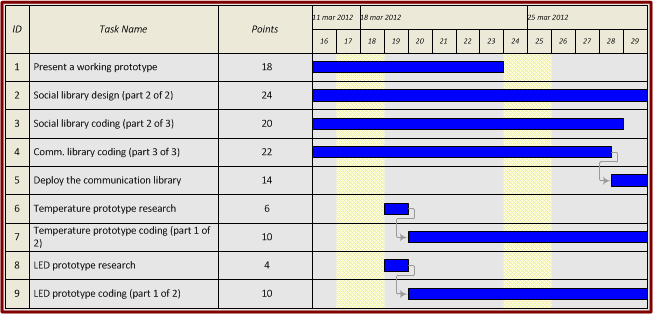
\includegraphics[scale=0.8]{img/sprints-gantt5.png}
\caption{Gantt diagram for the fifth sprint}
\label{fig:sprints-gantt5}
\end{figure}

\newpage

\section{Sprint 6}

Duration: 30/03 to 12/04\newline
Points total: 50

As this sprint coincided with Easter vacation, little was planned for this
sprint except some early work on the report and some coding for the Social
library and the Temperature prototype. Some team members left the city, others
left the country. No meetings with the customer were arranged. The team had a
brief, sort of 'unplanned' meeting right before the vacation during which they
were told that the hardware had not yet been ordered.

\begin{table}[ht!]
\begin{tabular}{ | r | l | c | c | r | }

\hline
\textbf{ID} & \textbf{Task} & \textbf{Points} & \textbf{Assigned to} & \textbf{Status} \\
\hline

1 & Work on the report						& 18 & Everyone & done \\
\hline
2 & Social library coding (part 3/3)		& 18 & E		& done \\
\hline
3 & Temp. prototype coding (part 2/2)		& 14 & B		& done \\
\hline

\end{tabular}
\end{table}

\begin{figure}[h!]
\centering 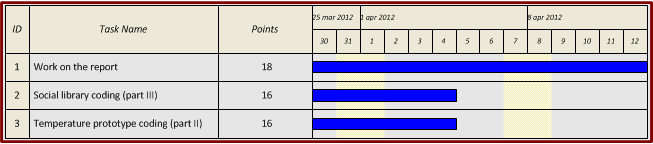
\includegraphics[scale=0.8]{img/sprints-gantt6.png}
\caption{Gantt diagram for the sixth sprint}
\label{fig:sprints-gantt6}
\end{figure}

\newpage

\section{Sprint 7}

Duration: 13/04 to 26/04\newline
Points total: 130

Back from Easter vacation! Roughly one week after the group was back from
Easter vacation, the necessary hardware components needed for the product had
arrived. Also the customer kindly provided a jacket that was to be
used for the final product. The various hardware devices were hooked up with the
Lilypad board and then tested individually, using a mockup application.

During this sprint the final product changed sightly from a T-shirt to a jacket.
The Lilypad board probably wasn't the best choice for a jacket product, in fact,
since the Arduino board could be hidden in a pocket, the team could have used
a smaller Arduino board, maybe with power connector and built-in battery
charger circuitry.

The Social library was finished, tested and an initial version deployed.
The Comm. lib started being thoroughly tested along with the prototypes.
Coding for the T-shirt application began. The Facebook and Twitter applications
started being converted from simple mockups to complete applications.

The team also worked on the delivery of the last supervised report.

\begin{table}[ht!]
\begin{tabular}{ | r | l | c | c | r | }

\hline
\textbf{ID} & \textbf{Task} & \textbf{Points} & \textbf{Assigned to} & \textbf{Status} \\
\hline

1 & Work on the report							& 22 & Everyone		& done \\
\hline
3 & T-Shirt app. coding (part 1/3)				& 22 & H			& done \\
\hline
2 & Build T-shirt prototype (part 1/3)			& 18 & AN,E,JH		& done \\
\hline
4 & Comm. library testing (part 1/2)			& 16 & AN,E,JH		& done \\
\hline
6 & Temp. prototype testing (part 1/2)			& 16 & B			& done \\
\hline
5 & Social library testing (part 1/2)			& 12 & E,H			& done \\
\hline
7 & Led prototype coding (part 2/2)				& 12 & AS			& done \\
\hline
8 & Facebook app. coding (part 1/2)				& 8  & E			& done \\
\hline
9 & Twitter application coding					& 4  & E			& done \\
\hline

\end{tabular}
\end{table}

\newpage

\section{Sprint 8}

Duration: 27/04 to 10/05\newline
Points total: 168

As the deadline for the project began closing near, the sprints started to be
more intensive. During this sprint the team had some problems with the hardware
which slowed down the development of the prototype. The LCD screen that the team
was using stopped working probably due to wrong wiring. The team received a
spare one that was in the Lab a few days before the end of the sprint. As the
T-shirt TUI changed into a jacket, the Lilypad board lost its main advantage
of being a sewable piece of hardware and the team started looking for alternative
Arduino boards, possibly with a battery socket and built-in recharge circuitry
which were missing in the Lilypad. Finally, a board with such features
(Arduino FIO) was chosen to substitute the Lilypad. A lot of testing involving
the Comm. lib was performed while building and testing the T-shirt prototype.
Testing was also performed for the other prototypes: Temperature and LED matrix.
The coding of the T-shirt and Facebook applications continued.
The T-shirt application couldn't be completed in time and was moved to the next
sprint. During one of the meetings, the customer liked an application that we
were using for testing the prototype functionality during the meeting's
demonstration and suggested the team to improve it and incorporate it in the
final product. This was rather unexpected as that application was only intended
for testing purposes. However the team added the client's request to their goals
for the next and final sprint.

\begin{table}[ht!]
\begin{tabular}{ | r | l | c | c | r | }

\hline
\textbf{ID} & \textbf{Task} & \textbf{Points} & \textbf{Assigned to} & \textbf{Status} \\
\hline

 1 & Build T-shirt prototype (part 2/3)			& 24 & AN,E,JH		& prolonged \\
\hline
 5 & T-shirt app. coding (part 2/3)				& 24 & H			& prolonged \\
\hline
 2 & Build a working prototype (week 1)			& 16 & Everyone		& done \\
\hline
 3 & Build a working prototype (week 2)			& 16 & Everyone		& done \\
\hline
 13 & Integration testing (part 1/2)			& 16 & Everyone		& done \\
\hline
 4 & Comm. library testing (part 2/2)			& 16 & AN,JH,E		& done \\
\hline
 7 & Work on the report							& 14 & Everyone		& done \\
\hline
 8 & Temp. prototype testing (part 2/2)			& 10 & B			& done \\
\hline
 10 & Facebook app. coding (part 2/2)			& 8  & E			& done \\
\hline
 12 & Facebook application testing				& 8  & E,H			& done \\
\hline
 6 & Social library testing (part 2/2)			& 6  & E			& done \\
\hline
 9 & Led prototype testing (part 1/2)			& 6  & AS			& done \\
\hline
 11 & Twitter application testing				& 4	 & E			& done \\
\hline

\end{tabular}
\end{table}

\newpage

\section{Final sprint}

Duration 11/05 to 25/05\newline
Points total: 172

The final sprint, as in most software processes, was very intensive and aimed
to find as many errors as possible in the product.

The team continued in building the T-shirt TUI prototype and testing
the oSNAP and T-shirt applications, and the system as a whole.
The LCD screen that the team was provided wasn't designed to work with the
voltage the Arduino FIO board was operating at: there were problems adjusting
the contrast. After considering various solutions to the problem, the team
opted to leave it like that since even if the contrast was off the text on the
display could still be read. During the first week the team held a presentation
of the product at a SINTEF office near the university. The presentation went
smoothly and the client seemed satisfied with the product. Since most of the
tasks for this sprint had to be completed before the presentation, the second
week was focused mostly on documentation work.


\begin{table}[ht!]
\begin{tabular}{ | r | l | c | c | r | }

\hline
\textbf{ID} & \textbf{Task} & \textbf{Points} & \textbf{Assigned to} & \textbf{Status} \\
\hline

 6 & Work on final report delivery				& 28 & Everyone	& done \\
\hline
 1 & Build T-shirt prototype (part 3/3)			& 24 & AN,E,JH	& completed \\
\hline
 5 & oSNAP application testing					& 24 & AN,E,JH	& done \\
\hline
 2 & T-Shirt app. coding (part 3/3)				& 18 & H		& completed \\
\hline
 4 & oSNAP application coding					& 18 & JH		& done \\
\hline
 9 & Integration testing (part 2/2)				& 16 & Everyone	& done \\
\hline
 3 & T-Shirt application testing 				& 14 & E,H		& done \\
\hline
 8 & System testing								& 12 & Everyone	& done \\
\hline
 7 & oSNAP WWW pages (market)					& 10 & JN		& done \\
\hline
10 & Led prototype testing (part 2/2)			& 8  & AS		& done \\
\hline
11 & Prepare a presentation for SINTEF & 8  & Everyone       & done \\
\hline
12 & Present to SINTEF & 1  & Everyone       & done \\
\hline

\end{tabular}
\end{table}

\newpage

\begin{figure}[h!]
\centering 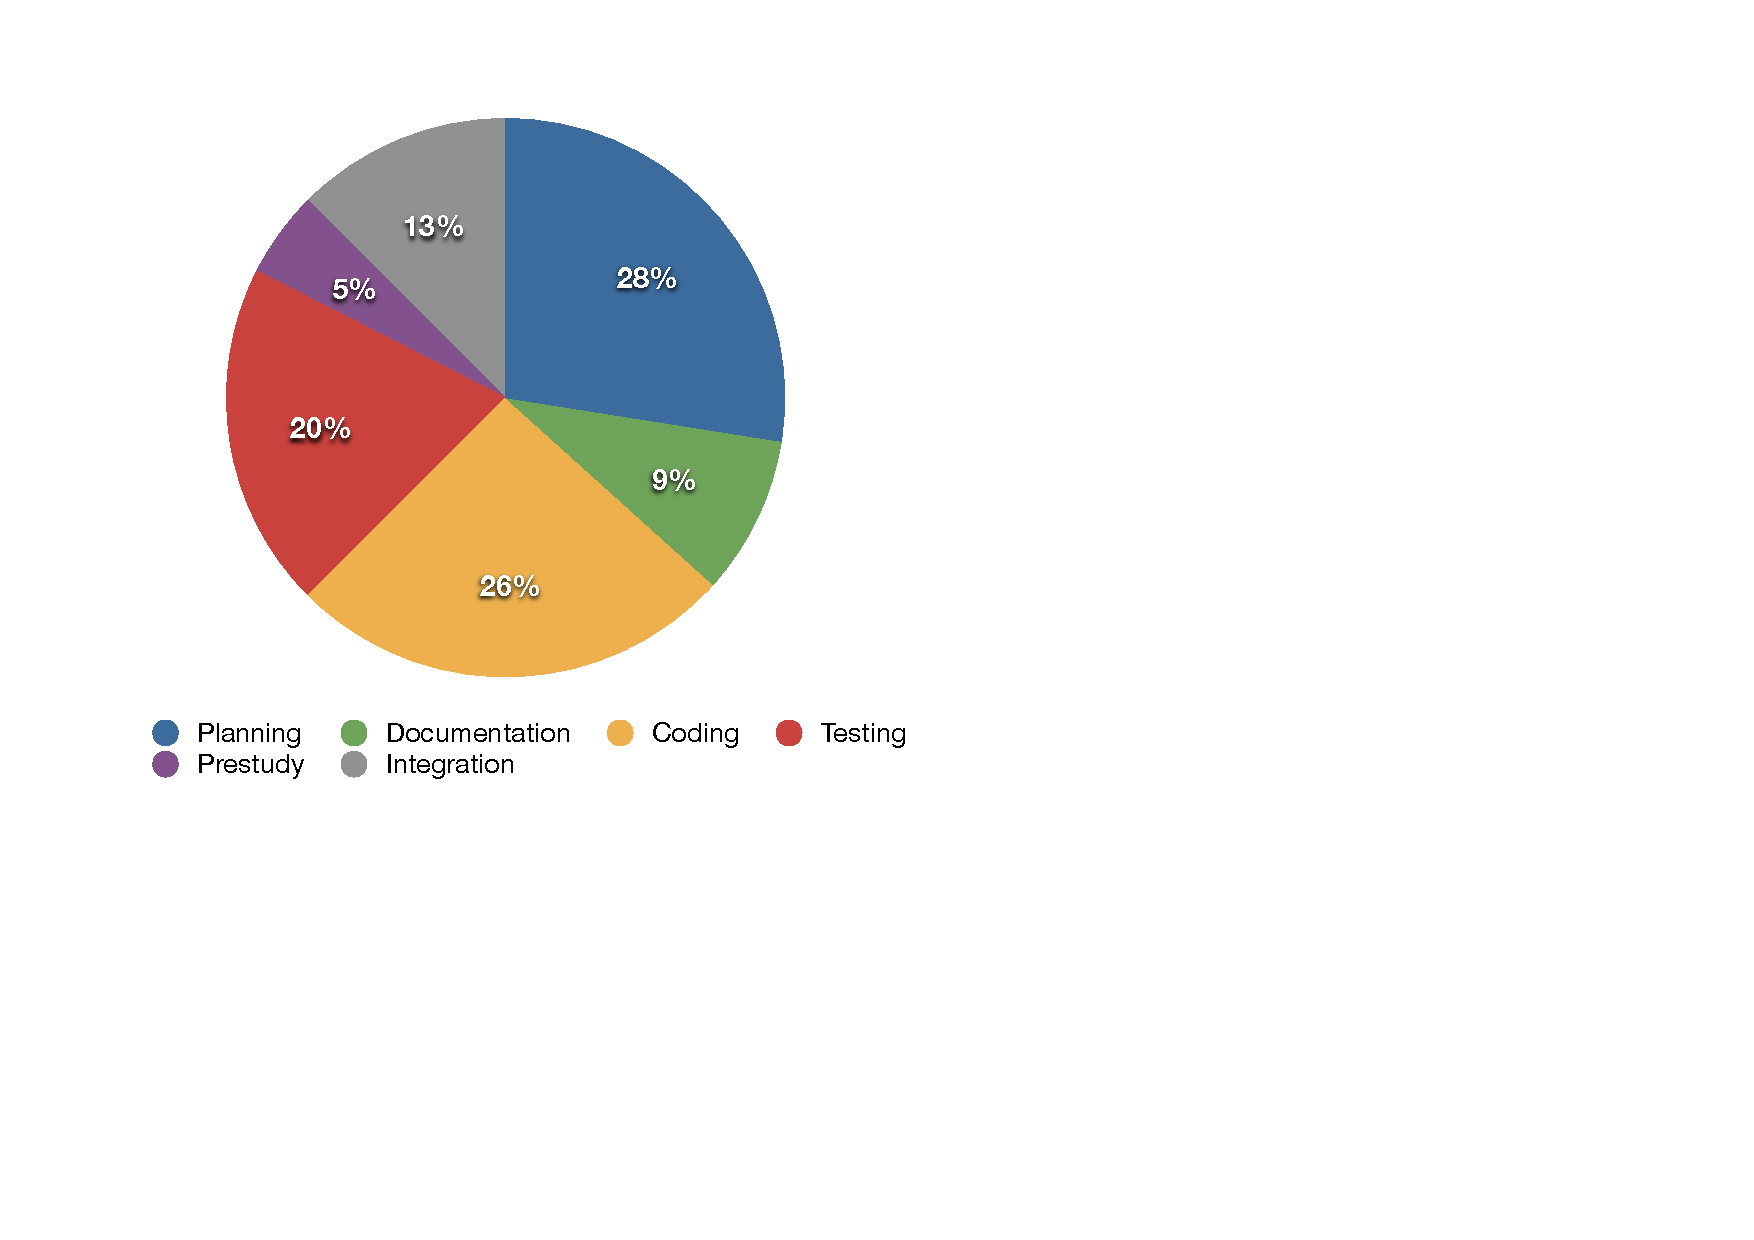
\includegraphics[scale=0.8]{img/pie_chart.pdf}
\caption{Story points breakdown}
\label{fig:sprints-points}
\end{figure}


\cleardoublepage
\chapter{Testing}\label{ch:systest}

Testing is an integral part of every development process.
In iterative software development processes, testing is usually planned in the
early stages of each iteration and planned as soon as the iteration itself is
complete. As the system evolves so does the testing; it should be more
comprehensive and cover not only modules but also the system itself as a whole.

\section{Testing approach}
Testing can be performed in a top-down or bottom-up fashion.

The top-down approach consists in integrating modules incrementally, moving
downward in the hierarchy in either a breadth-first or depth-first fashion. \newline
Subordinate dummy modules (stubs) are substituted one at time with the real ones
and tested. Regression testing follows each integration increment.

On the other side the bottom-up approach begins testing atomic modules,
sometimes combining them into clusters, and moves upward in the program
structure. Sometimes 'driver' programs are produced in order to test \newline
non-standalone components like libraries. This approach eliminates the need for
dummy modules, but the system as whole doesn't exist as an "entity" until the
last module is integrated.

In our case, since we presented many prototypes to the customer, we needed to
have an implementation of the system as a whole quite early. We coded various
mockup applications that acted as 'drivers' in order to demonstrate and test the
functionalities of the libraries. Stubs (or dummy modules) were also coded
to supply functionalities not yet fully implemented.

Some of these 'driver' programs were included in the source coded repository. 
These mockup programs were organized into a own package (see section \ref{section:mockup}).

\section{Customer feedback}
Receiving a constant feedback from the customer was very important as the
project didn't really have a specific set of requirements from the beginning.
Many prototypes were presented during meetings with the customer in order to
test the features implemented so far, receive a general acceptance on our
iteration goals and plan the next iteration. Feedback from the customer
allowed us to understand the most common use case scenarios and from those
obtain a set of requirements used to design the system and plan test cases.
Customer's feedback and proved to be very valuable for the project.

\section{Testing strategy}

\subsection{Unit testing}
Unit testing involves testing small portions of code or of the system itself
(modules). Where possible, functions have been tested indepentently. In order to
test non indipendent system modules, such as the libraries, mockup (driver)
applications were coded.

\subsection{Integration testing}
Once the system modules were completed they were integrated one by one into the
final system. After each stub/driver had been swapped with its correspective
module, it was tested again to ensure it was working properly.

\subsection{System testing}
System testing constists in testing the system as a whole.
In our case this consisted in testing our final prototype, performing a series
of tests involving all the parts of the system from the Android applications
to the hardware components.

\subsection{User interface testing}
Since our product encompassed various Android applications, we performed some
user interface testing. To make sure the user interfaces are understandable and
easy to use, we have delegated their testing to group members that have not been
involved in their design and coding.

\section{Functional requirement testing}
Since the project is a combination of proof-of-concept and research project,
tests are planned in order to test the functionality of the various parts of the
system against their own requirements and not for particular scenarios or more
specific use cases.

Tests were performed in order: the hardware and libraries were tested first
(the Android applications depended on both) and then integrated into more
complete tests involving all the parts of the TUI. prototype: Android
applications, libraries and the Arduino hardware.


\begin{table}[h!]
\begin{tabular}{|l|p{10cm}|}
\hline Test ID: &		[F1] Social lib. / [F5] Facebook app. / [F6] Twitter app.\\
\hline Purpose: &		Testing the Social library and social applications
						functionality \\
\hline Precondition: &	A mockup TUI prototype application is installed on an
						Android mobile, as well as the FB and Twitter apps. \\
\hline
Steps:
 & 1: Start the Facebook application \\
 & 2: Press 'Login' button \\
 & 3: Enter user's credentials and proceed with log in \\
 & 4: Exit the Facebook application \\
 & 5: Start the Twitter application \\
 & 6: Exit the Twitter application \\
 & 7: Start the mockup prototype application \\
 & 8: Press 'Discover social services' button \\
 & 9: Press 'Make a request' button \\
\hline
Expected result:
 & User is correctly authenticated (Facebook) \\
 & The Facebook social service is discovered by the mockup app \\
 & The Twitter social service is discovered by the mockup app \\
 & The mockup app. receives the correct response based on the request made by
	both social networks \\
\hline
Actual Result:
 & Passed \\
\hline
\end{tabular}
\caption{Test F1/F5/F6}
\end{table}


\begin{table}[h!]
\begin{tabular}{|l|p{10cm}|}
\hline Test ID: &		[F7] T-shirt prototype \\
\hline Purpose: &		Test T-shirt prototype functionality \\
\hline Preconditions: & The Arduino is connected to a PC via USB, all components
						are connected to the Arduino board; the Arduino board is
						on.\\
\hline
Steps:
 & 1: Toggle a LED status \\
 & 2: Send a signal to the vibrator module \\
 & 3: Print some text to LCD display \\
 & 4: Send sound to speaker \\
\hline
Expected result:
 & LED is toggled on/off \\
 & Vibrator works \\
 & Correct text is displayed on LCD \\
 & A sound is emitted by the speaker \\
\hline
Actual Result:
 & Passed \\
\hline
\end{tabular}
\caption{Test F7}
\label{tbl:f7test}
\end{table}


\begin{table}[h!]
\begin{tabular}{|l|p{10cm}|}
\hline Test ID: &		[F9] Temperature prototype \\
\hline Purpose: &		Test temperature prototype functionality \\
\hline Precondition: &	The Arduino board is connected to a PC via USB and
						turned on; the temperature sensor and a LCD screen are
						connected to the Arduino \\
\hline
Steps:
 & 1: Press a hardware button \\
\hline
Expected result:
 & Temperature is displayed on Arduino's LCD \\
\hline
Actual Result:
 & Passed \\
\hline
\end{tabular}
\caption{Test F9}
\label{tbl:f9test}
\end{table}


\begin{table}[h!]
\begin{tabular}{|l|p{10cm}|}
\hline Test ID: &		[F11] LED matrix. \\
\hline Purpose: &		Test LED matrix prototype functionality \\
\hline Precondition: &	The Arduino is connected to a PC via USB, and turned on;
						the LED matrix is connected to the Arduino. \\
\hline
Steps:
 & 1: Send sample data to Arduino \\
\hline
Expected result:
 & Correct LED light up according to sample data \\
\hline
Actual Result:
 & Passed \\
\hline
\end{tabular}
\caption{Test F11}
\label{tbl:f11test}
\end{table}


\begin{table}[h!]
\begin{tabular}{|l|p{10cm}|}
\hline Test ID: &		[F11] LED matrix prototype / [F10] LED matrix app. /
						[F2] Comm. library \\
\hline Purpose: &		Testing the LED matrix prototype and application \\
\hline Precondition: &	LED matrix applications is installed on the mobile and
						the Arduino board is powered \\
\hline
Steps:
 & 1: Pair cell phone with Arduino board using Android OS \\
 & 2: Start LED matrix application \\
 & 3: Select light in the matrix to adjust\\
 & 4: Change colour for the specified LED \\
\hline
Expected result:
 & 1: Correct LED is lighted up with the correct colour\\
\hline
Actual Result: &  Passed \\
\hline
\end{tabular}
\caption{Test F11/F10/F2}
\label{tbl:f11f10f2test}
\end{table}


\begin{table}[h!]
\begin{tabular}{|l|p{10cm}|}
\hline Test ID: &		[F8] Temperature app. / [F1] Social Lib / [F2] Comm. lib \\
\hline Purpose: &		Test the Temperature prototype and application
						functionality  \\
\hline Precondition: &	The two apps are installed and Arduino board is powered
						and paired. \\
\hline
Steps:
  & 1: Start Facebook application \\
  & 2: Press 'Log in' button \\
  & 3: Exit the Facebook application \\
  & 3: Start prototype's application \\
  & 4: Tap the screen to read the temperature\\
  & 5: Press button on the Arduino board to send temperature \\
\hline
Expected result:
  & Temperature is corretly read by the prototype and posted on the logged-in
	user's Facebook wall \\
\hline
Actual Result:
  & Passed \\
\hline
\end{tabular}
\caption{Test F8/F1/F2}
\label{tbl:f8f1f2test}
\end{table}


\begin{table}[h!]
\begin{tabular}{|l|p{10cm}|}
\hline Test ID: &		[F3] oSNAP app. / [F2] Comm. lib \\
\hline Purpose: &		Test connecting to the T-shirt TUI prototype using the
						Comm. lib and oSNAP application \\
\hline Precondition: &	The oSNAP app is installed on an Android phone; the
						Arduino board is installed in the T-shirt and powered. \\
\hline
Steps:
 & 1: Start oSNAP application \\
 & 2: Press 'Scan QR code' button \\
 & 3: Scan QR code on the T-Shirt \\
 & 4: Press 'Toggle LED' button (turn on) \\
 & 5: Press 'Toggle LED' button (turn off) \\
 & 6: Press 'Play sound' button \\
 & 7: Press 'Print "Hello world" button' \\
 & 8: Press 'Vibrate' button \\
\hline
Expected result:
 & The oSNAP application connects to the Arduino \\
 & Led is toggle on and then off \\
 & A sound is emitted \\
 & The vibration module vibrates \\
 & The 'Hello world' string is printed on the LCD \\
\hline
Actual Result:
 & Passed \\
\hline
\end{tabular}
\caption{Test F3/F2}
\end{table}


\begin{table}[h!]
\begin{tabular}{|l|p{10cm}|}
\hline Test ID: &		[F1] Social lib. / [F2] Comm. lib. / [F4] T-shirt app. /
						[F5] Facebook App / [F7] T-shirt TUI prototype \\
\hline Purpose: &		Test T-shirt prototype functionality \\
\hline Precondition: &	The two applications are installed and the T-shirt TUI.
						is on and paired with cell phone \\
\hline
Steps:
  & 1: Start Facebook application \\
  & 2: Press 'Log in' button \\
  & 3: Exit the Facebook application \\
  & 4: Start T-shirt app \\
  & 5: Press 'Discover services' button \\
  & 6: Select 'Facebook' from the list of available social services \\
  & 7: Set up rules to define the behavior of the tshirt \\
  & 8: Press 'Connect to Arduino' button \\
  & 9: Press 'Enable service' button \\
  &10: Exit the T-shirt application \\
\hline
Expected result:
   & Depending on the rules that have been set, the correct text is displayed,
   or the correct LED lights up.. and so on \\
\hline
Actual Result:
  &  Passed \\
\hline
\end{tabular}
\caption{Test F1/F2/F4/F5/F7}
\label{tbl:f1f2f4f5f7test}
\end{table}



\cleardoublepage
\chapter{Conclusion and Further Work}\label{ch:conclusion}
\section{Conclusion}
The final scope of the project was much bigger than we originally planned and envisioned. This large scope
was mainly caused because of all the different prototypes we had to implement. Originally we had planned
to implement one prototype with accompanying application, but ended up creating two developer libraries
along with 3 prototypes and 6 different Android applications in addition to a webpage for distribution of oSNAP
compatible software. While challenging this was also a lot of fun. We had a lot of freedom in developing
these products in the way we liked.

The weekly meetings with the customer proved to be very valuable and
a good way for the customer to keep track of progress. We showed the fruits of the work from the earlier
week to the customer and he could steer us in the direction he desired and comment on the results.


\section{Mistakes and new Experiences}
A big part of projects like this is reflecting back and see which mistakes were made throughout
the project lifetime. We can then learn why these mistakes happened and develop strategies to
prevent them from happening in future projects. This section describes the various pitfalls and
mistakes that were made throughout the project and what we learned from these.

\subsection{Establishing project requirements}
A lot of time was lost by prematurely starting the design and planning phase before the
requirements were properly understood and established. This was also caused by the shifting 
requirements that the customer had every meeting. We should have properly established a list of
requirements and agreed with the customer that these were the final requirements. In addition we
should have not started major planning, setting up resource management before the requirements
were properly set after a few meetings with the customer.

\subsection{Hardware problems}
There were various issues with the hardware for our prototypes. A big one was the large delay
from when we initially ordered the hardware and until we received them. The two months it took
for the hardware to arrive meant that in that period we could not do any integration and testing.
This was a major setback to our plans and this time was mostly spent writing documentation, planning
and testing the libraries for bugs. In addition the hardware we received was either wrong or not
optimal for our specifications. This was caused by miscommunication within the project group. In
addition we had not ordered backup or spare parts, so when for example the LCD screen broke,
we had to find other workarounds to solve this issue. In hindsight we should have made sure that
the list of hardware orders was correct and ordered additional spare parts in case something broke
or malfunctioned.

\subsection{Group meetings}
A chronic problem inside the group was late attendance to internal team meetings. For various reasons members of
the group would meet hours later than the agreed or planned time. This was somewhat mitigated to having 
the meetings later in the day and working into the late hours of the night.

\subsection{Limiting project scope}
Another problem caused by an early design choice was the level of portability. Initially we coded our libraries to support as wide range of platforms as possible (PC, Android, iOS, etc.). This caused various generalizations and concepts that worked not very well with Android. One prevalent example was callbacks and threads inside the Android system. While our library was based on multi-threading and callbacks through an observer pattern, this does not work on Android Java the same way one would expect on a PC. Since every prototype and testing software we coded was based on the Android platform this caused major problems and we had to spend a lot of time rewriting and redesigning libraries. So our choice of portability caused many problems considering the customer explicitly stated that we only needed to support Android. While portability is usually a good thing, the product quality should not suffer if it is not a high priority requirement.

\section{Further Work}
This section describes ideas, code and features we did not have time or resources to
finish at the project deadline. The section can also describe various interesting concepts 
that we visualized that we might have explored given more time.

\subsection{Supporting more communication technologies in ComLib}
Currently the ComLib only supports Bluetooth connections. Further work would be
to add support for additional communication technologies such as WiFi and Near Field 
Communication (NFC). The ComLib has been implemented so that this work should
be as easy as possible. Simply extend the Protocol class and implement the input and
output communication and the implementation should be fully forward and backwards
compatible with other versions of the ComLib.

\subsection{Supporting additional Social networks}
The SocialLib currently supports Twitter and Facebook. Support for additional social
networks like Google Plus, LinkedIn or MySpace was planned as future work. Also the
SocialLib has been implemented to accommodate this process as simple as possible
for the developer.

\subsection{Multi-Platform}
The Bluetooth part of the ComLib has been implemented using Android SDK. This means 
the Bluetooth part of the library will only run on an Android platform. The ComLib protocol
itself however, has been designed to support any type of platform. This means the ComLib
could be expanded to support other types of platform such as Bluetooth on iOS. This
should preferably be implemented as a common interface, so the developer only has to use
Bluetooth and the ComLib itself figures out if to use the Android version or the iOS version of
the Bluetooth Protocol.

\subsection{Security}
Currently the ComLib offers no level of security. Anyone with the mac address can connect
and have access to the full functionality of each prototype device. A future possibility could
be to define a security standard in the ComLib protocol like authentication with a password.


%\cleardoublepage
%\chapter{Bibliography}\label{ch:bibliography}
%Bibliography section
%Use \cite along with the label in curly brackets {} to citate one of our references
%for example: \cite{hp:computer-arch}
\begin{thebibliography}{99}
\bibitem{book:software-engineering} Sofware Engineering {\em Ian Sommerwille - Software Engineering 8th Edition 2007}
\bibitem{link:android} Android Developer's Resource  {\em http://developer.android.com/guide/basics/what-is-android.html}
\bibitem{link:facebook-api} Facebook Graph API {\em http://developers.facebook.com/docs/reference/api/}
\bibitem{link:facebook-dev} Facebook Developer Pages {\em http://developers.facebook.com/}
\bibitem{link:arduino} Official Arduino Website {\em http://www.arduino.cc/}
\bibitem{link:git} GIT Fast Version Control System {\em http://git-scm.com/}
\bibitem{link:opensocial} OpenSocial 2.0.1 {\em http://opensocial-resources.googlecode.com/svn/spec/2.0.1/}
\bibitem{link:xp} Extreme Programming {\em http://www.extremeprogramming.org}
\bibitem{link:wiki} Wikipedia {\em http://www.wikipedia.org/ }
\bibitem{link:spiral} Spiral model image source {\em http://www.designingprojectmanagement.com}
\bibitem{link:likelight} Red Pepperland Blog on the \emph{Likelight} {\em http://redpepperland.tumblr.com/post/3785566578/let-your-likelight-shine}
\bibitem{link:opensocial} OpenSocial {\em http://docs.opensocial.org/display/OS/Home}
\bibitem{link:shinding} Shindig {\em http://shindig.apache.org/}
\bibitem{link:scrumdo} ScrumDo Development Tool {\em http://www.scrumdo.com}
\bibitem{link:netbeans} Netbeans {\em http://netbeans.org/}
\bibitem{link:eclipse} Eclipse {\em http://www.eclipse.org/}
\bibitem{link:sublimetext} Sublime Text {\em http://www.sublimetext.com/}
\bibitem{link:arduinodev} Arduino Development Environment {\em http://arduino.cc/en/Guide/Environment}
\bibitem{link:facebooksdk} Facebook SDK {\em https://github.com/facebook/facebook-android-sdk/}
\bibitem{link:androidsdk} Android SDK {\em http://developer.android.com/sdk/index.html}
\bibitem{link:rxtx} RxTx {\em http://rxtx.qbang.org/}
\bibitem{link:googledocs} Google Documents {\em https://docs.google.com/}
\bibitem{link:googlesketchup} Google Sketchup {\em http://sketchup.google.com/}
\bibitem{link:visio} Microsoft Visio {\em http://visio.microsoft.com/}
\bibitem{link:skype} Skype {\em http://www.skype.com/}
\bibitem{link:sintef} SINTEF Corporate website {\em http://www.sintef.no/home/About-us/}
\end{thebibliography}


\textbf{Disclaimer:}
All images, figures and graphics are created by the oSNAP project members (unless explecitly cited with the source)


%Glossary
\printglossary

% ---------------------------------------------------------------------------- %
% Report appendixes goes here
\appendix
\appendixpage
\addappheadtotoc

\cleardoublepage
\chapter{Status Reports}\label{app:statusreports}
\section{Status Reports}

\subsection{Week 4}

PROJECT 10 Open Source Network Arduino Platform(oSNAP)
SUMMARY STATUS REPORT
Week 4
1 Introduction
First weeks status report where major directional decisions will be explained.
2 Progress summary
The starting weeks work was mainly focused on identifying the specifics of our task and for
every group member to start individual research into possibilities in Arduino, Facebook APIs,
other social network APIs and then reporting it back to the group at our meetings. Together we
tried to find good concepts for the Tangible User Interface(TUI) product that we was going to
make. We had a meeting with the customer on the friday where we discussed our concepts. In
this meeting the customer voiced wishes for the project to go in a more general direction than
focusing on specific tangible end products. We was going to make a framework where creating
products with an Arduino chip was lessened in complexity both for the developer and the end
user.
We also got Arduino products(Bluetooth module etc) from Simone Mora from IDI.
3 Open / closed problems
The direction the project should pursue in regards to the TUI and platform choice became clear
on the meeting with the customer.
How well the Arduino chip could handle wireless connections(Bluetooth, WiFi or Zigby) is an
open problem.
4 Planned work for next period
In the meeting with the customer we decided on a task for the next period. If we could show that
the Arduino could be linked with an Android and/or PC through a wireless connection we could
further refine the requirements and goals of the project.
5 Updated risks analysis
Wireless connectivity; if the Arduino chip addon modules(called SHIELDS) for Bluetooth etc.
was too hard to implement we would have to reconsider wireless connectivity. We set the “get
wireless to work” deadline to be one month. Otherwise we would have to use only cabled
connections and that would be clumsy on a lot of cool concepts.
Likelihood: 4 Impact: 6 Importance: 24

\subsection{Week 5}

PROJECT 10 Open Source Network Arduino Platform(oSNAP)
SUMMARY STATUS REPORT
Week 5
1 Introduction
A report of a very productive week with some breakthroughs and setbacks.
2 Progress summary
We started of by working on the tasks set forth. The bluetooth module(SHIELD) we got to
work much faster than we planned for so we set the bar higher and started working on a
general protocol to be used for communication between Arduino and computers regardless
of technology(USB,BT,WiFi etc). We also had people work on getting a working Facebook
application fetch data from Facebook(last post on Facebook wall). Getting a bluetooth
connection between Android and Arduino was also a challenging task that we got working by
the end of the week. Our results this week was presented to the customer on the friday as
we had agreed on. Our progress relative to our plan is very good, we are actually ahead of
schedule.
We also started working on the preliminary report that is due in WEEK 6. We chose to write this
in LaTeX language as this is the most powerful way to customise the style of our report.
In the meeting with the customer we had to revise our plan regarding to the Android framework.
The way social networks/applications connect to our framework should be with intents(an
Android standard) and the framework should be highly flexible in regards to which applications
can work on it. This lead us to reject some of the code we had made for Facebook fetching,
Android Bluetooth talking amongst other things.
We also established working process management tools in GitHub and
ScrumDo(www.scrumdo.com).
3 Open / closed problems
Closed: wireless connectivity to Arduino is a reality and Bluetooth was decided upon as this is a
standard in all mobile smart phones these days so the possibilties are bigger.
Open:
The concept of intents on Android needs to be understood and tried in action.
4 Planned work for next period
Revise established plans on all levels of our project.
Set the plans in motion.
5 Updated risks analysis
The risk of wireless connectivity not working is void after this weeks progress.

\cleardoublepage
\chapter{First draft of the architecture}\label{app:firstdraftarchi}
The client asks for a Java framework that works on either Android or desktop, to support the connection between a Arduino board and social services.

If a programmer wants to use the framework to connect a social service to the Arduino board, he would like to work with data in either end and forward it.

\begin{itemize}
  \item\textbf{Example 1:} 

  He would like to retrieve data from the social service, do something with it, and push data to the Arduino.

  \item\textbf{Example 2:}

  He would like to grab data from the Arduino, do something with it, and upload it to a social service.
\end{itemize}

This illustrates a split in the middle where the developer wants to treat the data himself. Since there is no direct connection between a social service and the Arduino board from our framework, it makes sense to split the framework into two parts.

\begin{itemize}
  \item\textbf{Framework part one:} Retrieving and uploading data between social service and Java.
  \item\textbf{Framework part two:} Grab and push data between the Arduino board and Java.
\end{itemize}

Both frameworks would need to support Android and development. This is an advantage for us who is going to create the framework, and for those who are going to use it.

The disadvantage is that it will be no direct connection from the Arduino board to a social service.
I.e, the board can not connect directly through the Internet to Facebook. It needs a middleman, either an Android phone or a laptop.

After some tests, we have figured out that it makes no difference if the Arduino board is connected through a Bluetooth device or trough an USB cable. If it's an USB cable, the board shows up as a COM port. If the board is paired with the computer/mobile using the operating system/Android, it also shows up as a COM port. So the program searches the COM ports and connects to the board anyhow. (It may not work on all bluetooth chipsets)


The board needs a firmware that is precompiled on a computer.
That process should be easy for the developer.

\begin{figure}
  \centering
  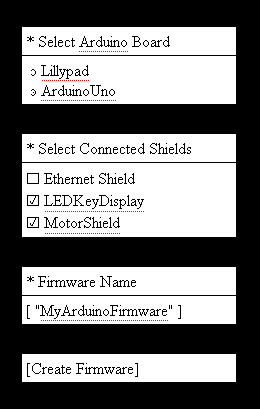
\includegraphics{./img/architecture-mockupgui.png}
  \caption{An early mockup of the GUI}
  \label{fig:architecture-mockupgui}
\end{figure}

On Create Firmware it should be compiled a file that the developer implements in his Arduino program.

\section{Example run framework part 1}

How the developer connects to the board on Android/PC after pairing the Arduino with the system.

\javacode
\begin{lstlisting}
//We search the COM ports trying to find the board
Arduinoboard board = Arduinoboard.findBoard();

//We retrive the current firmware name onboardString currentFirmware = board.getFirmwareName();

if(currentFirmware.equals("MyArduinoFirmware"){
    //Everything is OK, the firmware we want is on board.
}
else{
    //There is wrong Firmware/no firmware
    //We upload the one we precreated on our computer.
    File file = new File("/firmwareLocation/firm.fw");
    ArduinoFirmware fw = ArduinoFirmware.getFW(file);

    board.uploadFirmware(fw);
}

//We can see what shields we have according to the premade firmware
ArduinoShield shields = board.getShields();

//Or we can ask for the shield directly
LEDKeyPadShield display = board.getShield(LEDKeyPadShield.class);

//Now the developer can do what he wants with the shields.
display.printText("HelloWorld");
\end{lstlisting}

\clearpage

\begin{figure}[hp]
  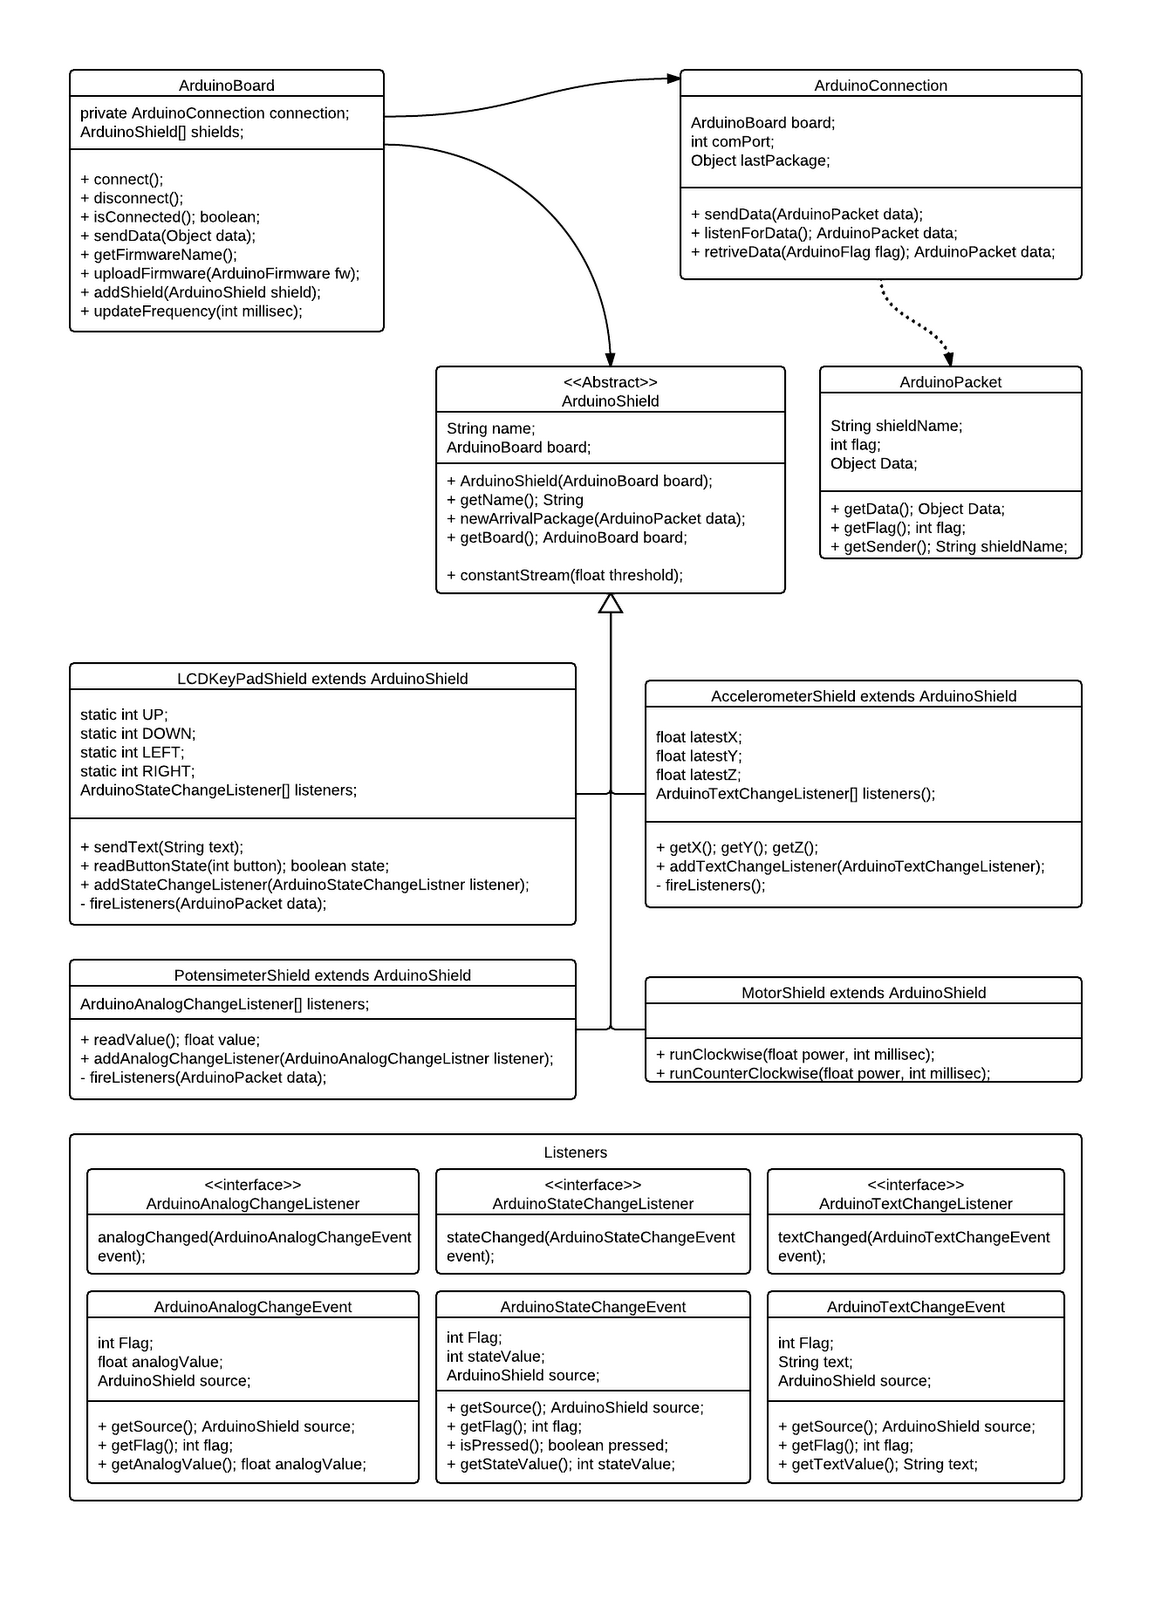
\includegraphics{./img/architecture-arduinojava.png}
  \caption{A first sketch of Arduino-Java connection}
  \label{fig:architecture-arduinojava}
\end{figure}

\section{Adding a listener to shield}


Developer adds his listener.
\javacode
\begin{lstlisting}
LEDKeyPadShield display = board.getShield(LEDKeyPadShield.class);
display.addStateChangeListener(new ArduinoStateChangeListener(){
  @Override
   public void stateChanged(ArduinoStateChangeEvent event) {
    if(event.getFlag == LEDKeyPadShield.DOWN){
        //Get down and boogie
    }
   }
});
\end{lstlisting}

In ArduinoConnection we have listenForData(); method, that has its own thread listening on it.

Steps:
listenForData() recives a ArduinoPacked data from Arduino board.

Thread looks in board.shields to find the same board as packet.getName().

It dumps the package into the shield.newArrivalPackage(dataPackage);

It is then up to the shield class to extract the data from package, and fire off an ArduinoEvent to the listeners.


\section{Constant data stream solutions}

Some shields, like the accelerometer is sensitive and will always send data to the program. On a mobile phone who constantly needs to work on these packages this will be straining on the battery.

The constantStream threshold value is a signal to the ArduinoBoard to indicate how often in will update.

Threshold = 0.0f; means all data will be streamed
Threshold = 1.0f; means no data will be send from shield to the program. You can only retrieve data by specifically asking for it.

A mid value is dependent on the Shields connected, if the accelerometer has upper values in x,y,z directions from $<-1000, 1000>$, a threshold of $0.8f$ indicates we need extreme sudden change of $\Delta(0.8*2000)$ in one of the x,y,z axis to send a notification from the Arduino board.

Example, extremely sudden change (In one cycle?) from -700 to +800 in x direction.  

It's not yet clear if we can implement this function into the firmware.

\section{Example run framework part 2}

\javacode
\begin{lstlisting}
//In this case, we register our service with a premade simple Facebook app we have created on
//Facebook.com
SocialService service = new FacebookService(FacebookSevice.getAppAuth("appName"));

//The initateLogin will call up a browser window and request user to log in
//(automatically handle the calls depending if its called from Android or PC)
service.initateLogin();

//Adding listener
service.addSocialListener(new SocialListener(){
  @Override
   public void newPost(Post post) {
    String message = post.message[0];
   }
});

//New post
service.postNewPost(new Post("Hello Profile"));
\end{lstlisting}

\cleardoublepage
\chapter{Meeting reports}\label{app:meetings}
%\newcommand{\Date}{}



\section{Date: 20/01/2012}

\textbf{Participants:} Everyone

\textbf{Agenda} 
\begin{itemize}
\item First meeting, 
\item Contact the client 
\item Contacted the client

\begin{itemize}
\item First meeting at Friday 27/01 at 14:00 
\end{itemize}
\item Send mail to the client with phone numbers/names 
\item Checking free slots in schedule when we can have meetings

\begin{itemize}
\item (Monday 12:15 and out) 
\item (Entire Wednesday) 
\item (Friday 14:15 and out) 
\end{itemize}
\end{itemize}
\textbf{To do to next meeting:}

Check solutions for connecting Facebook and Arduino\\
 $Facebook->openSocial(Java)->C/AarduionIDE->Chipset$ 
\begin{itemize}
\item Everyone

\begin{itemize}
\item BrainStorm 
\item Make some notes/schemes. 
\end{itemize}
\item Henrik

\begin{itemize}
\item Read on OpenSocial 
\end{itemize}
\item Jonas

\begin{itemize}
\item Setup GIT, Mailing list, examine OpenSocial and Shindig 
\end{itemize}
\item Emanuele

\begin{itemize}
\item Find available Facebook APIs, document on Open Social, Apache Shindig.. 
\end{itemize}
\item Asbjørn

\begin{itemize}
\item Read on Arduino 
\end{itemize}
\item Anders and Bjørnar

\begin{itemize}
\item Connect arduino to java 
\end{itemize}
\item Johan

\begin{itemize}
\item OpenSocial, Java -\textgreater{} Arduino 
\item Send two mail 
\item To SINTEF 
\item To reception to book room Friday 4th floor at 14:15 every week 
\end{itemize}
\end{itemize}
\textbf{Next meeting:}

Monday 23/01 GreenHouse\\
 Discuss brainstorm/possiblities\\
 Get a meeting room at Friday at 14, to meet with the client 


\end{document}

